\chapter{First-order reversal curve diagram modelling of framboidal greigite}
\label{ch:res-4}

\section*{Abstract}
In this chapter...\par

\section{Introduction}
Introduction goes here...\par

\section{Methodology}
\subsection{The micromagnetic method}
A ferromagnetic (in the broad sense, i.e., including ferrimagnetic behaviour) material has a Gibbs free-energy functional (excluding the effects of thermal fluctuations and magnetostriction) which can be written as \citep{Brown}:
\begin{equation}
E_\text{G} = \int_{\Omega} (\phi_{\text{exchange}} + \phi_{\text{anisotropy}} + \phi_{\text{stray}} + \phi_{\text{external}})\,\text{d}^3 \boldsymbol{r},
\end{equation}
where $\Omega$ is the ferromagnetic volume and $\text{d}^3 \boldsymbol{r}$ the volume differential, so integrations is carried out over the ferromagnetic body. Here,
\begin{equation}
\phi_{\text{exchange}}=A|\nabla\boldsymbol{m}|^2,
\end{equation}
where $\boldsymbol{m}$ is the reduced (unitary) magnetisation vector and $A$ the exchange stiffness constant, is an expression providing a continuum approximation of the energy density due to quantum-mechanical exchange forces between atomic spins \citep{Landau1935}.
\begin{equation}
\phi_{\text{anisotropy}}=\frac{K_1}{2}\sum_{i\neq j}\gamma_i^2\gamma_j^2 + K_2\prod_i\gamma_i^2,
\end{equation}
where $\gamma_i$ denote the direction cosines and $K_1,K_2$ the first and second magnetocrystalline (MCA) anisotropy constants, respectively, is the MCA energy density for cubic-anisotropic ferromagnets. In terms of the reduced magnetisation vector components this has the form:
\begin{equation}
\phi_{\text{anisotropy}}=K_1(m_x^2m_y^2+m_y^2m_z^2+m_z^2m_x^2),
\end{equation}
where $K_2$ has been neglected since in the cubic anisotropy system we are assuming, $K_1$ is the dominant term at room temperature. The magnetic Gibbs free-energy associated with the magnetostatic self-interaction of the ferromagnetic body and the stray magnetic field $\boldsymbol{H}_{\text{stray}}$ it produces is given by:
\begin{equation}
\phi_{\text{stray}}=-\frac{\mu_0M_\text{S}}{2} \boldsymbol{m} \cdot \boldsymbol{H}_{\text{stray}}
\end{equation}
where $M_\text{S}$ is the saturation magnetisation and $\mu_0=4\pi \times 10^{{-}7}\,\text{T}\text{m}/\text{A}$ is the magnetic constant or vacuum permeability. Finally, the energy density due to the magnetostatic interaction of the ferromagnetic body and an external field $\boldsymbol{H}_{\text{external}}$ is:
\begin{equation}
\phi_{\text{external}}=-\mu_0 M_{\text{S}} \boldsymbol{m} \cdot \boldsymbol{H}_{\text{external}}.
\end{equation}

From thermodynamics, it is well known that under isothermal and isobaric conditions a system will be driven spontanteously toward an equilibrium state with locally minimal Gibbs free-energy. Micromagnetic algorithms aim to find the equilibrium magnetisation $\boldsymbol{m}$ by minimising the Gibbs free-energy functional \citep{Fischbacher2017}. Here, a modified gradient-descent method \citep{OConbhui2017} is used for this endeavour.\par

Numerical solutions require a discretisation of the spatial domain into a grid or \textit{mesh} with a finite number of points on which numerical solutions are calculated. In FEMs, three-dimensional space is decomposed into tetrahedral pieces called finite elements with the vertices of these elements called the nodes. On each of the mesh nodes, a unit vector is initially defined to create an initial guess; the micromagnetic algorithm then attempts to minimise the magnetic Gibbs free-energy by variating the orientation of each of these vectors while ensuring they remain unitary. In micromagnetic theory \citep{Brown} there are some linearisations, which means that there should not be large variations in the direction of $\boldsymbol{m}$ between neigbouring nodes. For unconstrained micromagnetic models it is expected that the microstructure will contain nouniform structures at least to some degree. To model nonuniform structures it is sufficient that the spatial discretisation in the model is always smaller than the exchange length $l_\text{exch} = \sqrt{2A/\mu_0M_\text{S}^2}$ \citep{Rave1998}, which for greigite is $l_\text{exch} \approx 6.6\, \text{nm}$; a maximum element size of 5$\nm$ has been chosen for all the meshes. The non-local problem of calculating the stray field is handled via a hybrid finite-element/boundary-element formulation \citep{Fredkin1990}.\par

\subsection{The FORC model}
Ferromagnetic materials have magnetisation states that are dependent on their magnetic (or thermal, chemical) history. This is the well-known phenomenon of magnetic hysteresis \citep{Mayergoyz1986}. Standard hysteresis measurements proceed by saturating the magnetisation by applying a saturating magnetic field $\boldsymbol{B}=\mu_0\boldsymbol{H}$ with strength $B_{\text{sat}}$; in this saturated state, magnetisations are uniform and completely aligned with the applied field. Gradually, the magnetic field strength is decreased to desaturate the magnetic material. A curve $M=M(B)$ of the material's scalar magnetisation $M=\boldsymbol{M}\cdot\boldsymbol{\hat{n}}$ (where $\boldsymbol{\hat{n}}$ is a unit vector in the direction of the applied field) against the applied field strength $B$ is traced. When the applied field vanishes, the remanent state is obtained. The ratio of the remanent state magnetisation $M_{\text{RS}} \geq 0$ to the saturation magnetisation $M_{\text{S}}$ is one of the key magnetic hysteresis parameters \citep{Dunlop}. The applied magnetic field strength is then increased in the direction opposite the initial (effectively, making $B<0$): the applied field value at which a magnetisation $M=0$ state is obtained is called the coercivity $B_\text{C}$. If from this state the field is taken back to zero, a magnetisation $M>0$ is obtained; however, there exists a field value $B_{\text{CR}}<B_{\text{C}}$, called the coercivity of remanence, from which a remanent $M=0$ state is obtained for $B=0$. These fields and the ratio $B_{\text{CR}}/B_{\text{C}}$ are also key parameters characterising a hysteresis curve. To complete a hysteresis loop, the magnetisation is driven to a negatively saturated state and gradually returned to the initial positive saturation state. This traces the main (upper and lower) branches of a hysteresis loop.\par

A scatter plot of the ratio $M_{\text{RS}}/M_{\text{S}}$ against the ratio $B_{\text{CR}}/B_{\text{C}}$ is called a Day plot \citep{Day1977} and is one of the most typically used plots in rock magnetism \citep{Dunlop}. Although these basic magnetic hysteresis parameters can be useful to discern the magnetic domain state and magnetisation reversal mechanisms of magnetic systems, it has been shown recently that the Day plot can lead to erroneous interpretations \citep{Egli2014,Roberts2017}. It is logical that access to the interior of the hysteresis loop can reveal more information about magnetic behaviours, which is the basic idea behind the calculation of $B_{\text{CR}}$.\par

First-order reversal curves are a set of partial hysteresis curves obtained from magnetisation states on the upper branch of the hysteresis loop for different field values $B_a$. For a given $B_a$ and $M(B_a)$, the field $B=B_b$ is increased to positive saturation to trace a magnetisation curve. This proceedure for a number of $B_a$ values creates a magnetisation function on two variables $M=M(B_a,B_b)$ for $B_b \geq B_a$. The FORC distribution $\rho$ is then defined as \citep{Roberts2000}:
\begin{equation}\label{forc distribution}
\rho = -\frac{\mu_0^2}{2}\frac{\partial^2 M}{\partial B_a \partial B_b}.
\end{equation}
The FORC distribution is an empirical analog of the Preisach weight function which is well defined for magnetic systems that do not necessarily obey the strict conditions imposed by the Preisach model \citep{Mayergoyz1986}. Contour plots of the FORC distribution $\rho$ are called FORC diagrams and have been used increasingly as a proxy for the magnetic domain state and magnetic reversal behaviour of a variety of systems \citep{Pike1999,Pike2001,Roberts2000,Dumas2007,Egli2010,Egli2014,Biasi2016,Proenca2017,Zhao2017}.\par

Calculation of the FORC distribution (Eqn. \ref{forc distribution}) is performed by least-squares fitting of a second degree polynomial surface $M(B_a,B_b)=a_0 + a_1 B_a + a_2 B_b + a_3 B_a B_b + a_4 B_a^2 + a_5 B_b^2 + e$, where $e$ is a collection of error terms, on a subgrid of the magnetisation function $M(B_a,B_b)$ including ($2\times\text{SF}+1$)$^2$ points in the vicinity of $(B_a, B_b)$ as determined by the smoothing factor SF \citep{Pike1999}. If the magnetisation is approximated in this manner, calculation of Eqn. \ref{forc distribution} yields $\rho=-\mu_0^2 a_3 / 2$. Rotated $B_b,B_a$ axes, the so-called coercive field $B_c = (B_b - B_a)/2$ and interaction field $B_u = (B_a + B_b)/2$, respectively, are used for contour plots to produce FORC diagrams.\par

In an ensemble of randomly oriented particles, there are equal probabilities of finding particles with any orientation within an area element of the unit sphere. To simulate a randomly oriented dispersion of identical particles efficiently, it is necessary to obtain a number of applied field directions (equivalently, particle orientations with respect to the applied field) each of them representative of a given area on the unit sphere; additionally all these areas should span the unit sphere or alternatively, in high symmetry particle scenarios, a section of the sphere which can recreate the particle geometry under rotation operations \citep{ValdezGrijalva2017,ValdezGrijalva2018}. Given the symmetry of the model framboidal cluster geometry (Fig. \ref{FIG_01}) it is sufficient to simulate the effects of field orientations on the spherical triangle delimited by $(1, 0, 0), (a, a, a), (0, 0, 1)$, where $a=1/\sqrt{3}$. Then, the spherical triangle is subdivided into roughly equiareal triangle sub-units to obtain 85 triangular cells. The center of each cell represents a field orientation we obtain the FORC response for here. The average of the FORC response for all these orientations is the approximation to the FORC response of the ensemble of randomly oriented framboidal clusters.\par

Since these calculations are computationally intensive, it is important to reduce further the amount of calculations. For each field orientation, the upper branch of the hysteresis loop is calculated. Most of the curve is traced by the sum of reversible motions of the magnetisations in each of the individual particles in the framboid. Therefore, FORCs need only to be calculated for $B_a$ field values for which at least one particle undergoes an irreversible rotation (switching) \citep{ValdezGrijalva2017,ValdezGrijalva2018}. A saturating field $B_{\text{sat}}=250\mT$ and an external field rate of change of 2$\mT$ is used for all calculations. This means that for each field orientation we calculate 251 FORCs to obtain the FORC signal of a given cluster orientation.\par
\begin{figure}
\centering
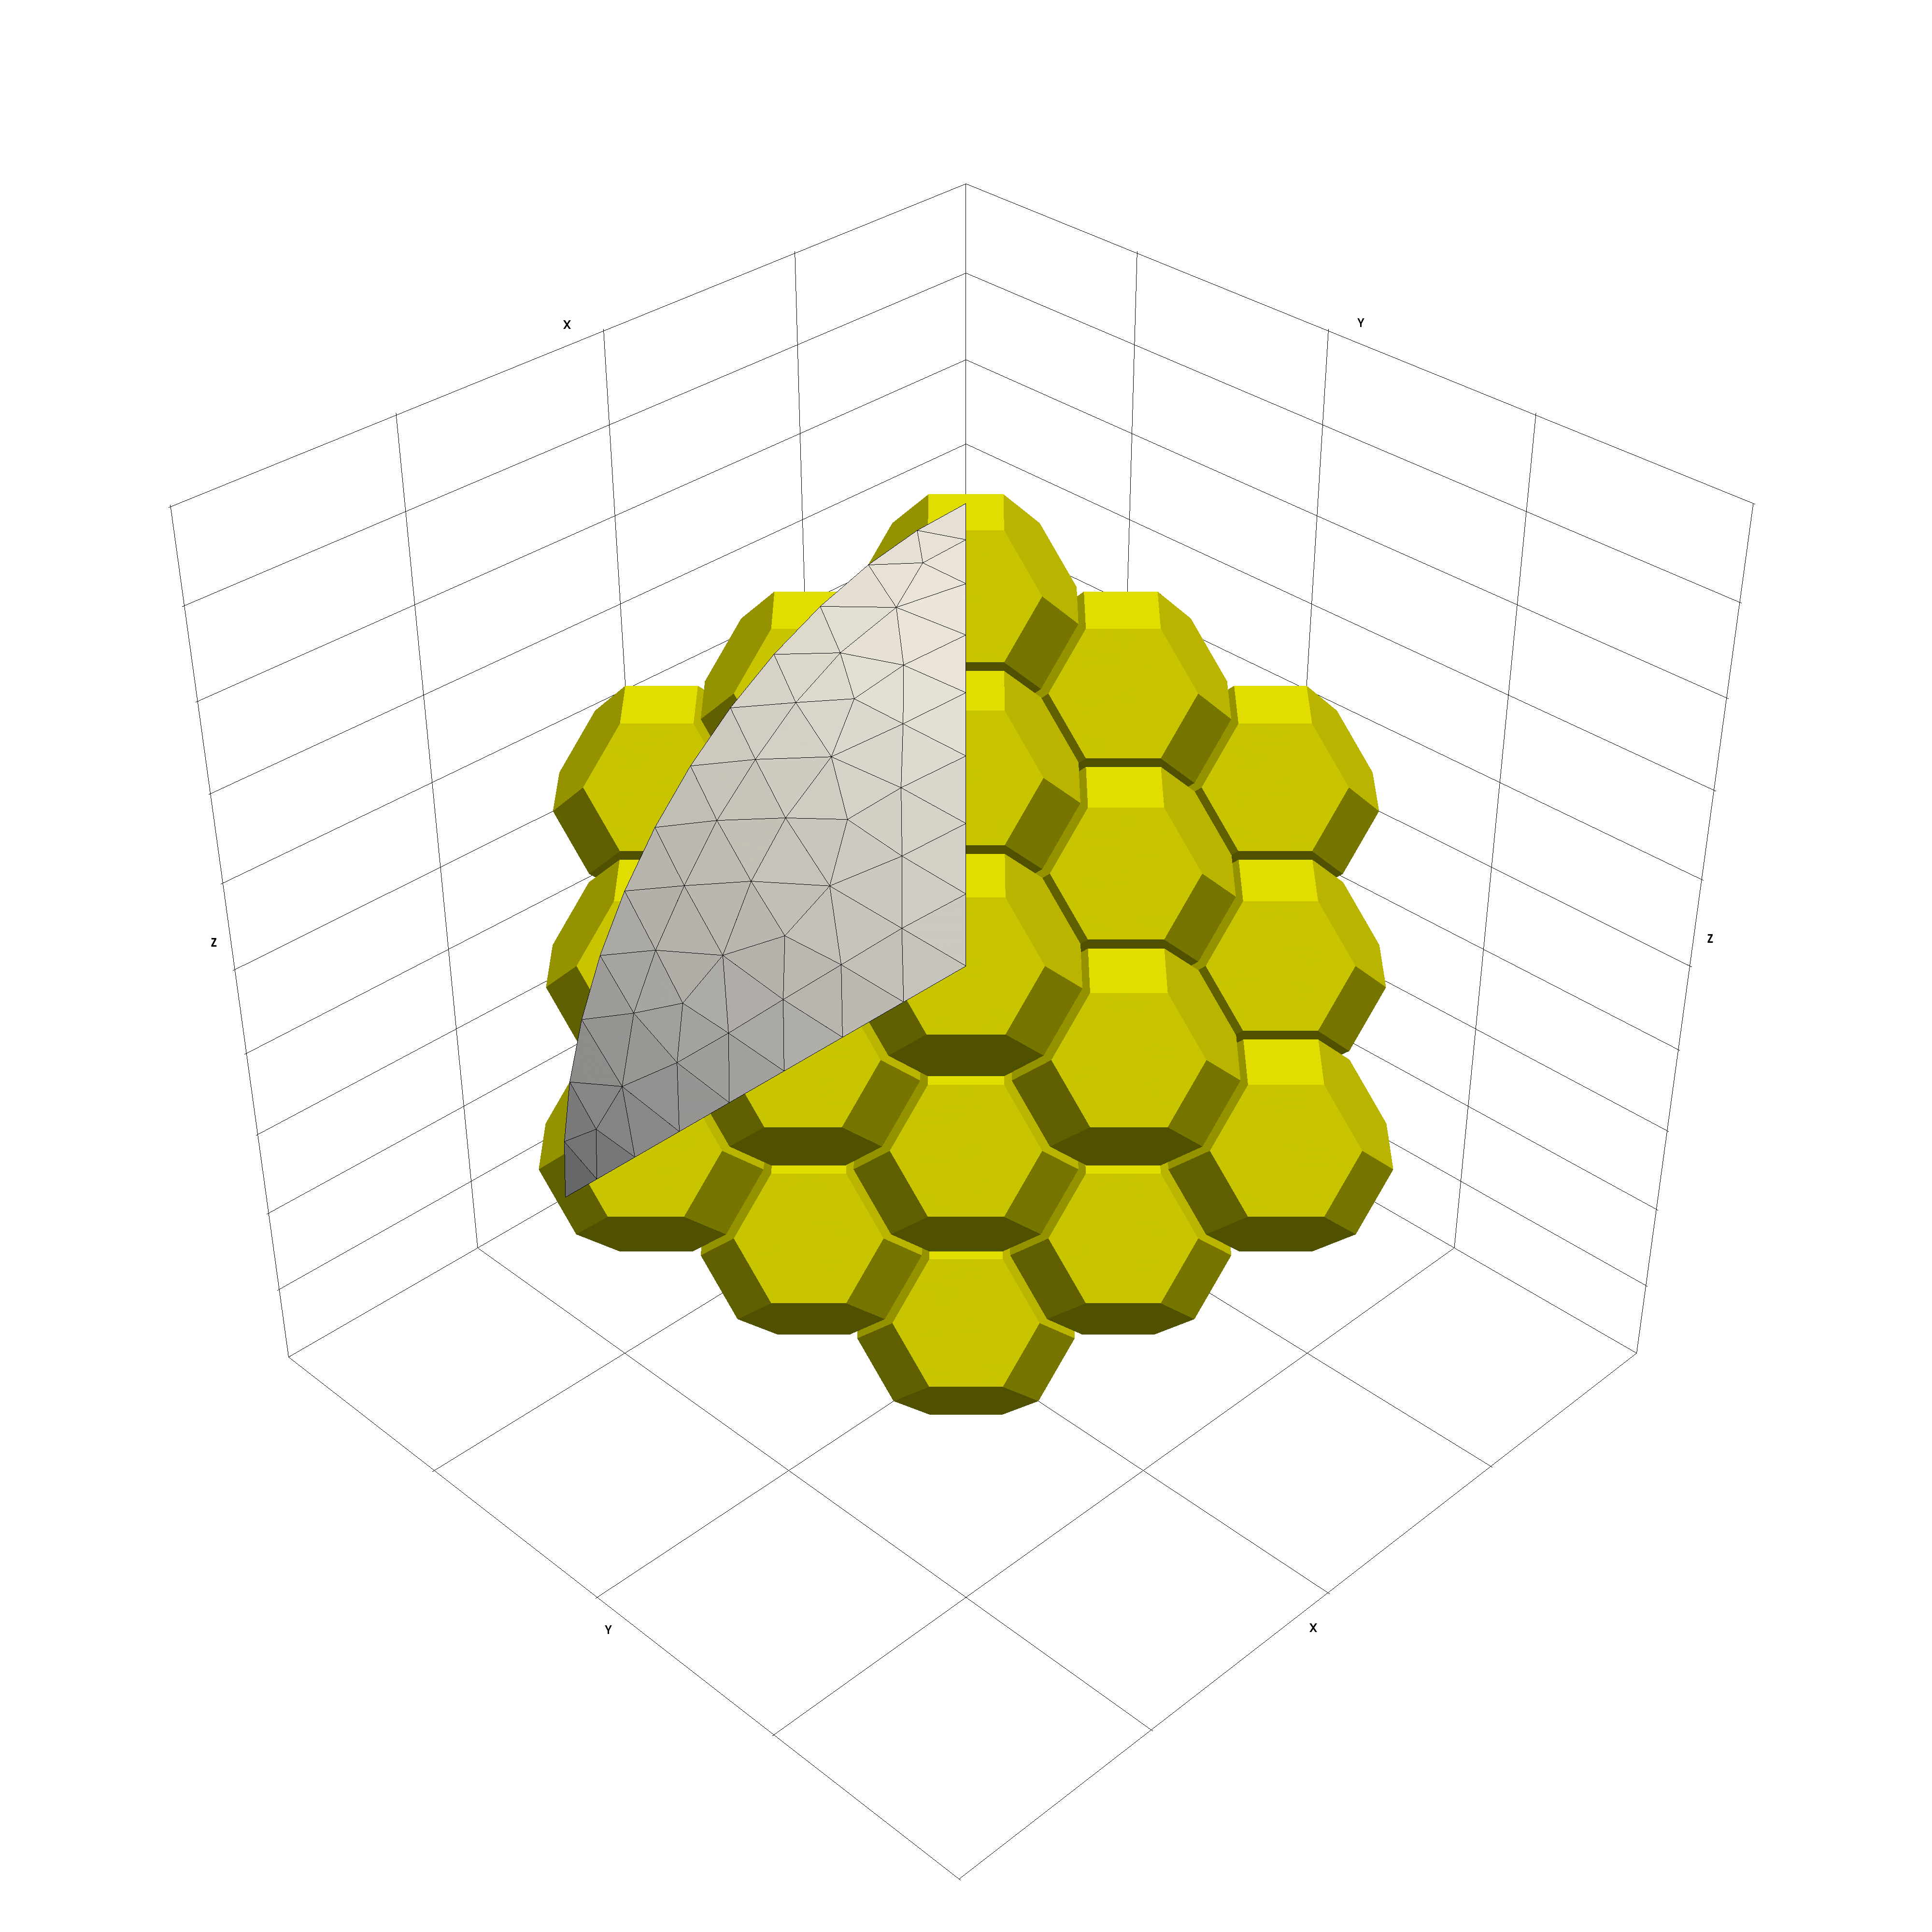
\includegraphics[width=\textwidth]{research-4/figs/mesh_orientations_HD.png}
\caption[Framboidal mesh and field orientations]{Framboidal mesh and field orientations.}
\label{FIG_01}
\end{figure}

\section{Results}
\subsection{The FORC diagrams}
The FORC response is dependent on field orientation with respect to the framboid. When the field is close to the isolated particle easy axis $<$111$>$, the hysteresis response of the framboid is saturated down to $\roughly 50\mT$ (Fig. \ref{FIG_02}a). Complex local interaction fields then cause outer particles to coherently rotate to minimise the stray fields as the field is decreased. All particles in the framboid remain in a SD state throughout the hysteresis and FORCs. The remanent state is a double magnetic super-vortex with a low remanence $\roughly 0.1 \, M_\text{S}$ which is due to the effective magnetic flux-closure brought about by the super-vortex structures.
\begin{figure}
\centering
\includegraphics[width=\textwidth]{research-4/figs/forcs_easy_hard.pdf}
\caption[FORCs when the field is along an easy and a hard axis]{FORCs when the field is along an easy and a hard axis}.
\label{FIG_02}
\end{figure}
\par

The FORC diagram for the easy axis-aligned applied field (Fig. \ref{FIG_02}b) has a positive peak at $B_c\approx 80\mT$ roughly 5$\mT$ above the $B_u=0$ axis. A negative response of comparable magnitude is situated below and to the left of the distribution peak. The positive peak response corresponds to the large upward jumps experienced by the reversal curve starting at the lowest switching field $B_a\approx{-}80\mT$ as it approaches positive saturation (Fig. \ref{FIG_02}a). The negative response is caused by irreversible switching of individual particles in the framboid on FORCs with higher $B_a$ values at $B_b\approx 75 \mT$. Most of the FORC diagram has a noisy appearance due to the complexity of individual particle responses caused by the local interaction fields. However, a large, continuous, positive response close to the $B_c=0$ axis is important as it was found for all field orientations.\par

When the applied field is close to a hard axis, the hysteresis and FORC response is very different. The hysteresis main branches are much more rounded, desaturating via reversible motion and experiencing the first irreversible switchings at roughly 150$\mT$ (Fig. \ref{FIG_02}c) which are much smaller than the jumps for the easy axis-aligned applied field response (Fig. \ref{FIG_02}a). The FORC diagram (Fig. \ref{FIG_02}d) is dominated by signals close to the $B_c=0$ axis.\par

Averaging the response for all 85 field orientations results in a very smooth set of FORCs (Fig. \ref{FIG_03}a). The remanence of the framboid ensemble is $M_\text{RS}/M_\text{S}\approx 0.1$ and the coercivity $B_\text{C}\approx 5\mT$; compare this to the remanence and coercivity of a noninteracting ensemble of isolated SD greigite particles, $M_\text{RS}/M_\text{S}\approx 0.86$ and $B_\text{C}\approx 24\mT$, respectively \citep{ValdezGrijalva2018}. The magnetostatic interactions between the particles in every framboid cause great decreases in the remanence and coercivity. The saturating field for the framboid ensemble is roughly 150$\mT$.
\begin{figure}
\centering
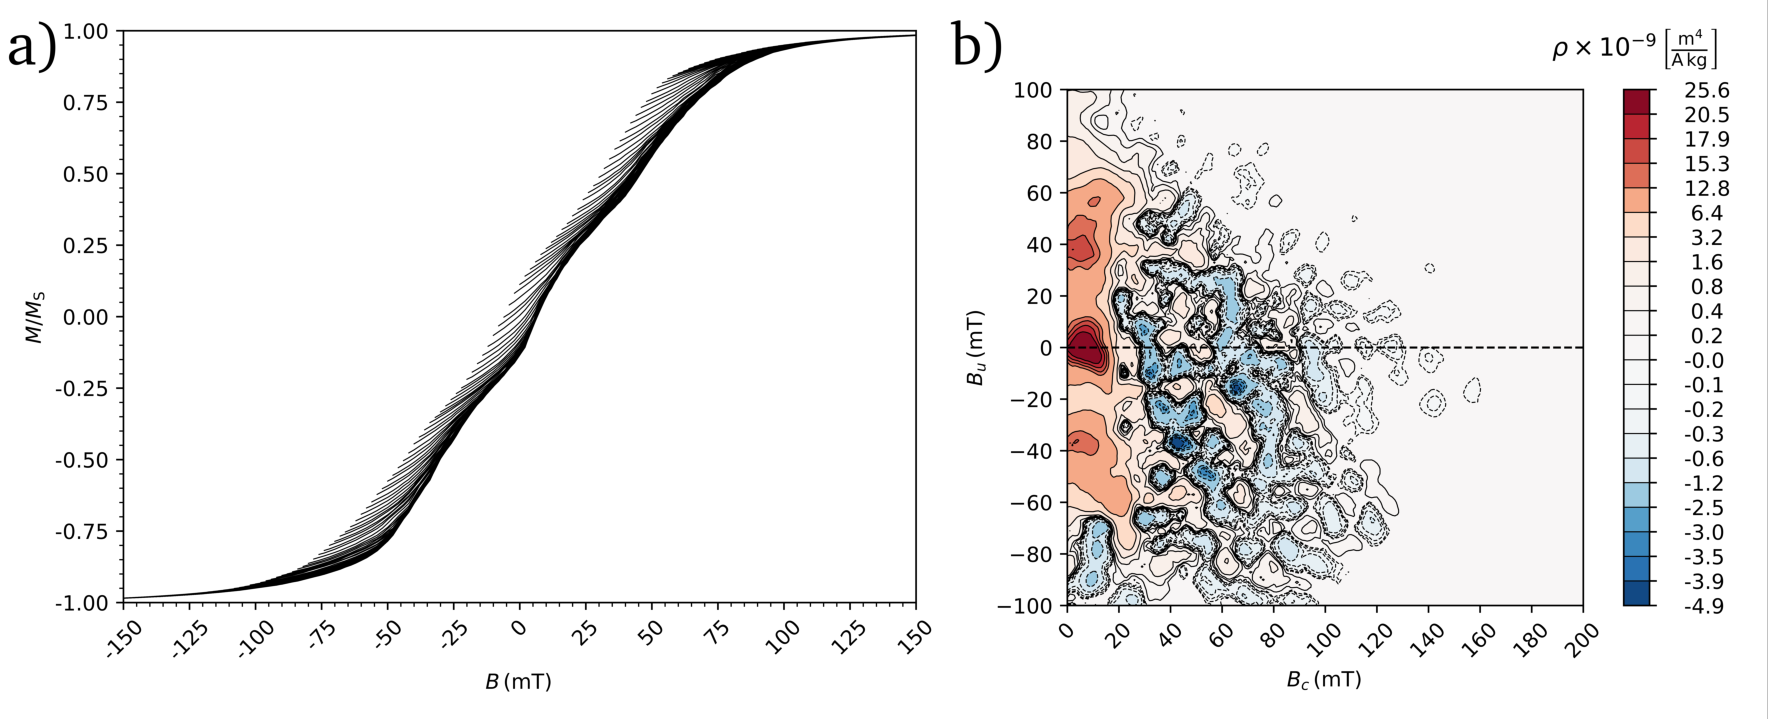
\includegraphics[width=\textwidth]{research-4/figs/forc_avg.pdf}
\caption[FORCs of the framboid dispersion]{FORCs of the framboid dispersion.}
\label{FIG_03}
\end{figure}
\par

The FORC diagram of the simulated ensemble of framboidal clusters (Fig. \ref{FIG_03}b) is dominated by a large response roughly centered at ($B_c=10\mT,B_u=0$) and two lobes roughly at ($B_c=10\mT,B_u=\pm 40\mT$). These sources are part of a larger, continuous signal roughly in the rectangle defined by coordinates ($B_c=0,B_u={-}60\mT$), ($B_c=20\mT,B_u={-}60\mT$), ($B_c=20\mT,B_u=100\mT$), ($B_c=0,B_u=100\mT$). This is because the set of averaged FORCs are very smooth and do not experience sharp discontinuities on the path tho positive saturation; therefore, the signal is dominated by the differences in magnetisation values along the upper branch that serve as starting points for the FORCs.\par

The negative and smaller positive responses form a noisy region to the right of this rectangle. However, these are only $\roughly 20 {\%}$ the magnitude of the peak response at maximum on some very small regions, and most of it is less than $\roughly 10 {\%}$. The simulated FORC response of an ensemble of randomly aligned greigite framboids (composed of 30$\nm$ particles) is much lower per mass than the response of noninteracting, isolated 30$\nm$ grains: 25.6$\times 10^{{-}9}\,\text{m}^4\text{A}^{{-}1}\text{kg}^{{-}1}$ and 531.6$\times 10^{{-}9}\,\text{m}^4\text{A}^{{-}1}\text{kg}^{{-}1}$ \citep{ValdezGrijalva2018} for the peak responses, respectively.\par

Using the model of \citep{ValdezGrijalva2018} the FORC response of noninteracting ensembles of isolated greigite particles in the size range 30--80$\nm$ is obtained to produce FORC diagrams of mixtures of framboidal greigite and isolated particles in the SD and SV magnetic domain states. FORC diagrams of mixtures of equal mass framboidal and noninteracting SD particles (Fig. \ref{FIG_04}a) and equal mass framboidal and noninteracting SV partices (Fig. \ref{FIG_04}b) are presented. The mixture of framboidal greigite and noninteracting SD particles (Fig. \ref{FIG_04}a) is dominated by the noninteracting SD signal, erasing most of the noisy region while keeping the important framboidal source close to the $B_c=0$ axis.
\begin{figure}
\centering
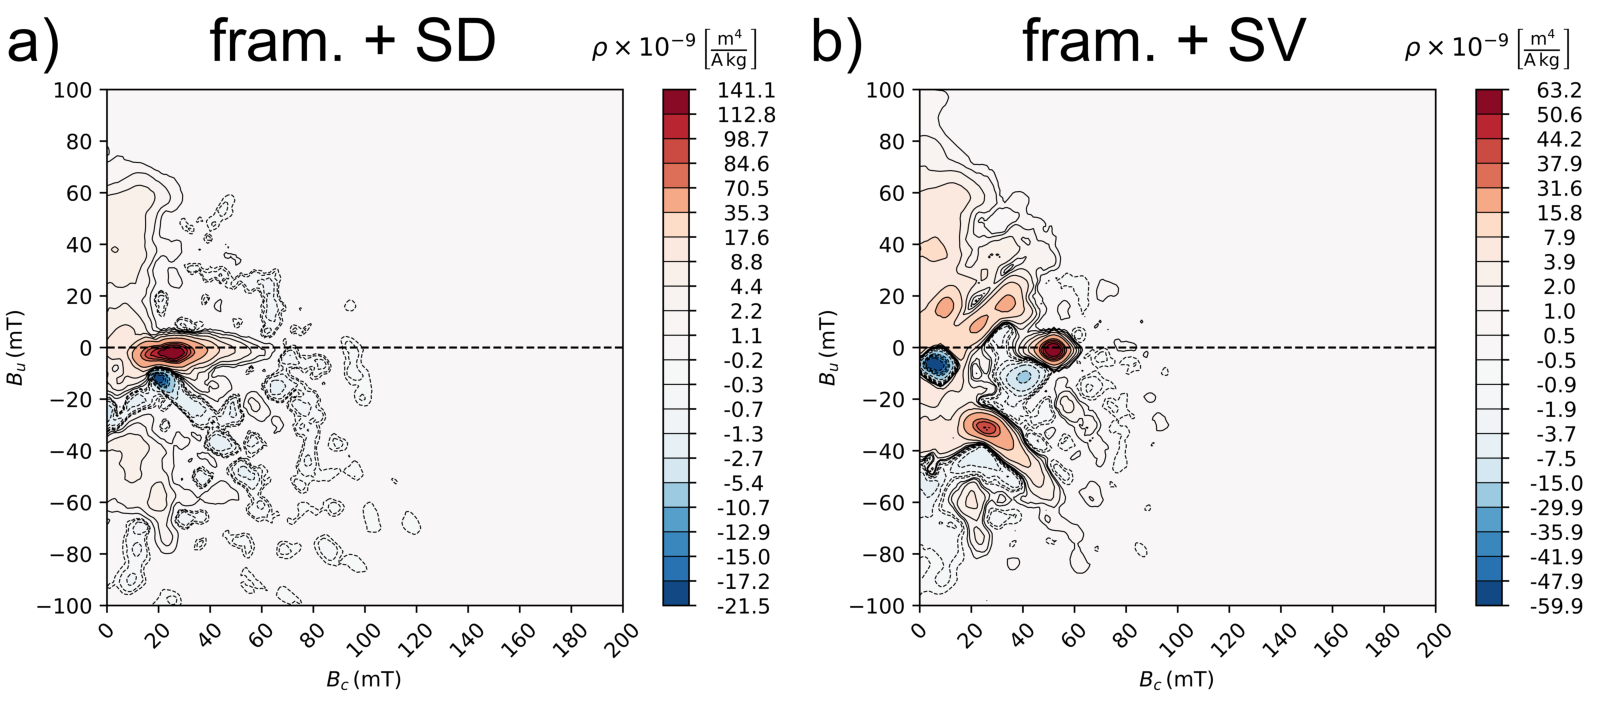
\includegraphics[width=\textwidth]{research-4/figs/forc_mix.pdf}
\caption[FORCs of a dispersion of framboids and noninteracting SD particles]{FORCs of a dispersion of framboids and noninteracting particles.}
\label{FIG_04}
\end{figure}
\par

When noninteracting SV particles are included (Fig. \ref{FIG_04}b) to the framboid signal, the response is dominated by the SV particles. As with the mixture of SD and framboidal greigite, most of the noisy region disappears on account of it being so faint and there is more complex interactions between the SV and framboidal signals in the region close to the $B_c=0$ axis as this is a region that is also responsive to the SV particles \citep{ValdezGrijalva2018}.\par

A scatter plot of the remanence of saturation $M_\text{RS}/M_\text{S}$ against the coercivity of remanence $B_\text{CR}$ to coercivity $B_\text{C}$ ratio, the so-called Day plot \citep{Day1977}, reveals the simulated ensemble of framboidal greigite in a region that is unoccupied by the noninteracting, isolated particles (Fig. \ref{FIG_05}), i.e., a region with a remanence as low as that of ensembles of SV particles $\roughly 80\nm$ but $B_\text{CR}/B_\text{C}$ values that are expected of smaller particles $\roughly 70\nm$ \citep{ValdezGrijalva2018}. Increasing content of SD or SV noninteracting particles have very different effects on the Day plot (Fig. \ref{FIG_05}): increasing the SD content increases the remanence and decreases the $B_\text{CR}/B_\text{C}$ ratio; whereas, increasing the SV content has little effect on the remanence while increasing the $B_\text{CR}/B_\text{C}$ value.\par
\begin{figure}
\centering
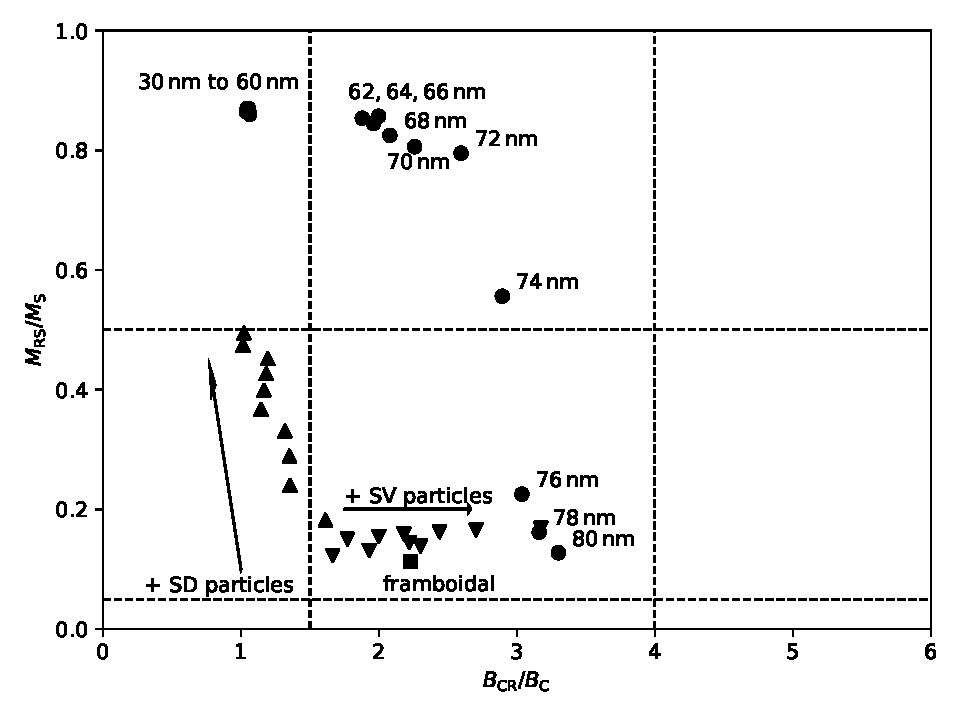
\includegraphics[width=\textwidth]{research-4/figs/DayPlot.pdf}
\caption[Day plot of framboid and noninteraring particles mixtures]{Day plot of framboid and noninteraring particles mixtures.}
\label{FIG_05}
\end{figure}
\par

\subsection{Hysteresis of larger particle framboids.}
Due to memory and time constraints, the FORC response of larger particle framboids was not simulated. However, hysteresis simulations of framboids composed of fifteen, larger $d=76\nm$ particles were carried out for a few selected field orientations. When the applied field is close to the easy axis the main branches remain saturated down to 50$\mT$ (Fig. \ref{FIG_06}), when some particles in the framboid nucleate vortices and change orientation (Fig. \ref{FIG_06}a). The remanent state (Fig. \ref{FIG_06}b) has a super-vortex structure in which most particles are individually in a two-domain state with very clearly defined domain walls (Fig. \ref{FIG_06}b, green). This state is remarkably similar to the easy-aligned SV state exhibited by large >200$\nm$ particles \citep{ValdezGrijalva2017B} with six domains curling around the vortex core. Noninteracting 76$\nm$ particles nucleate vortices \citep{ValdezGrijalva2018}; however, for this field orientation, the innermost particle in the cluster always remains in a SD state due to the internal magnetostatic interactions.
\begin{figure}
\centering
\includegraphics[width=\textwidth]{research-4/figs/loop21_76nm_annotated.pdf}
\caption[Hysteresis of a framboid with 76$\nm$ particles]{Hysteresis of a framboid with 76$\nm$ particles.}
\label{FIG_06}
\end{figure}
\par

\section{Discussion}
Discussion section...\par

\section{Conclusions}
Conclusion section...\par

%----------------------------------
\renewcommand\bibname{{References}}
\bibliographystyle{elsarticle-harv}
\bibliography{references}

%\subsection{Mesh generation}
%To generate close-packed arrangements of truncated octahedral particles
%Truncated octahedral geometry 
%Outline of mesh generation. Explain the algorithm to produce arbitrarily large ordered framboidal meshes.\par
%\subsection{Remanent states}
%The remanent states, micromagnetic solutions and electron holography maps. Explain about the remanent states and how they would appear under electron holography studies. Important to stress how the electron holography maps can be misleading as evidenced by Figs. \ref{FIG_21}, \ref{FIG_22}, \ref{FIG_23}, \ref{FIG_24}, \ref{FIG_25}, \ref{FIG_26} which show either a single-vortex or a two-vortex structure depending on the angle of the beam.\par
%\begin{figure}
%\centering
%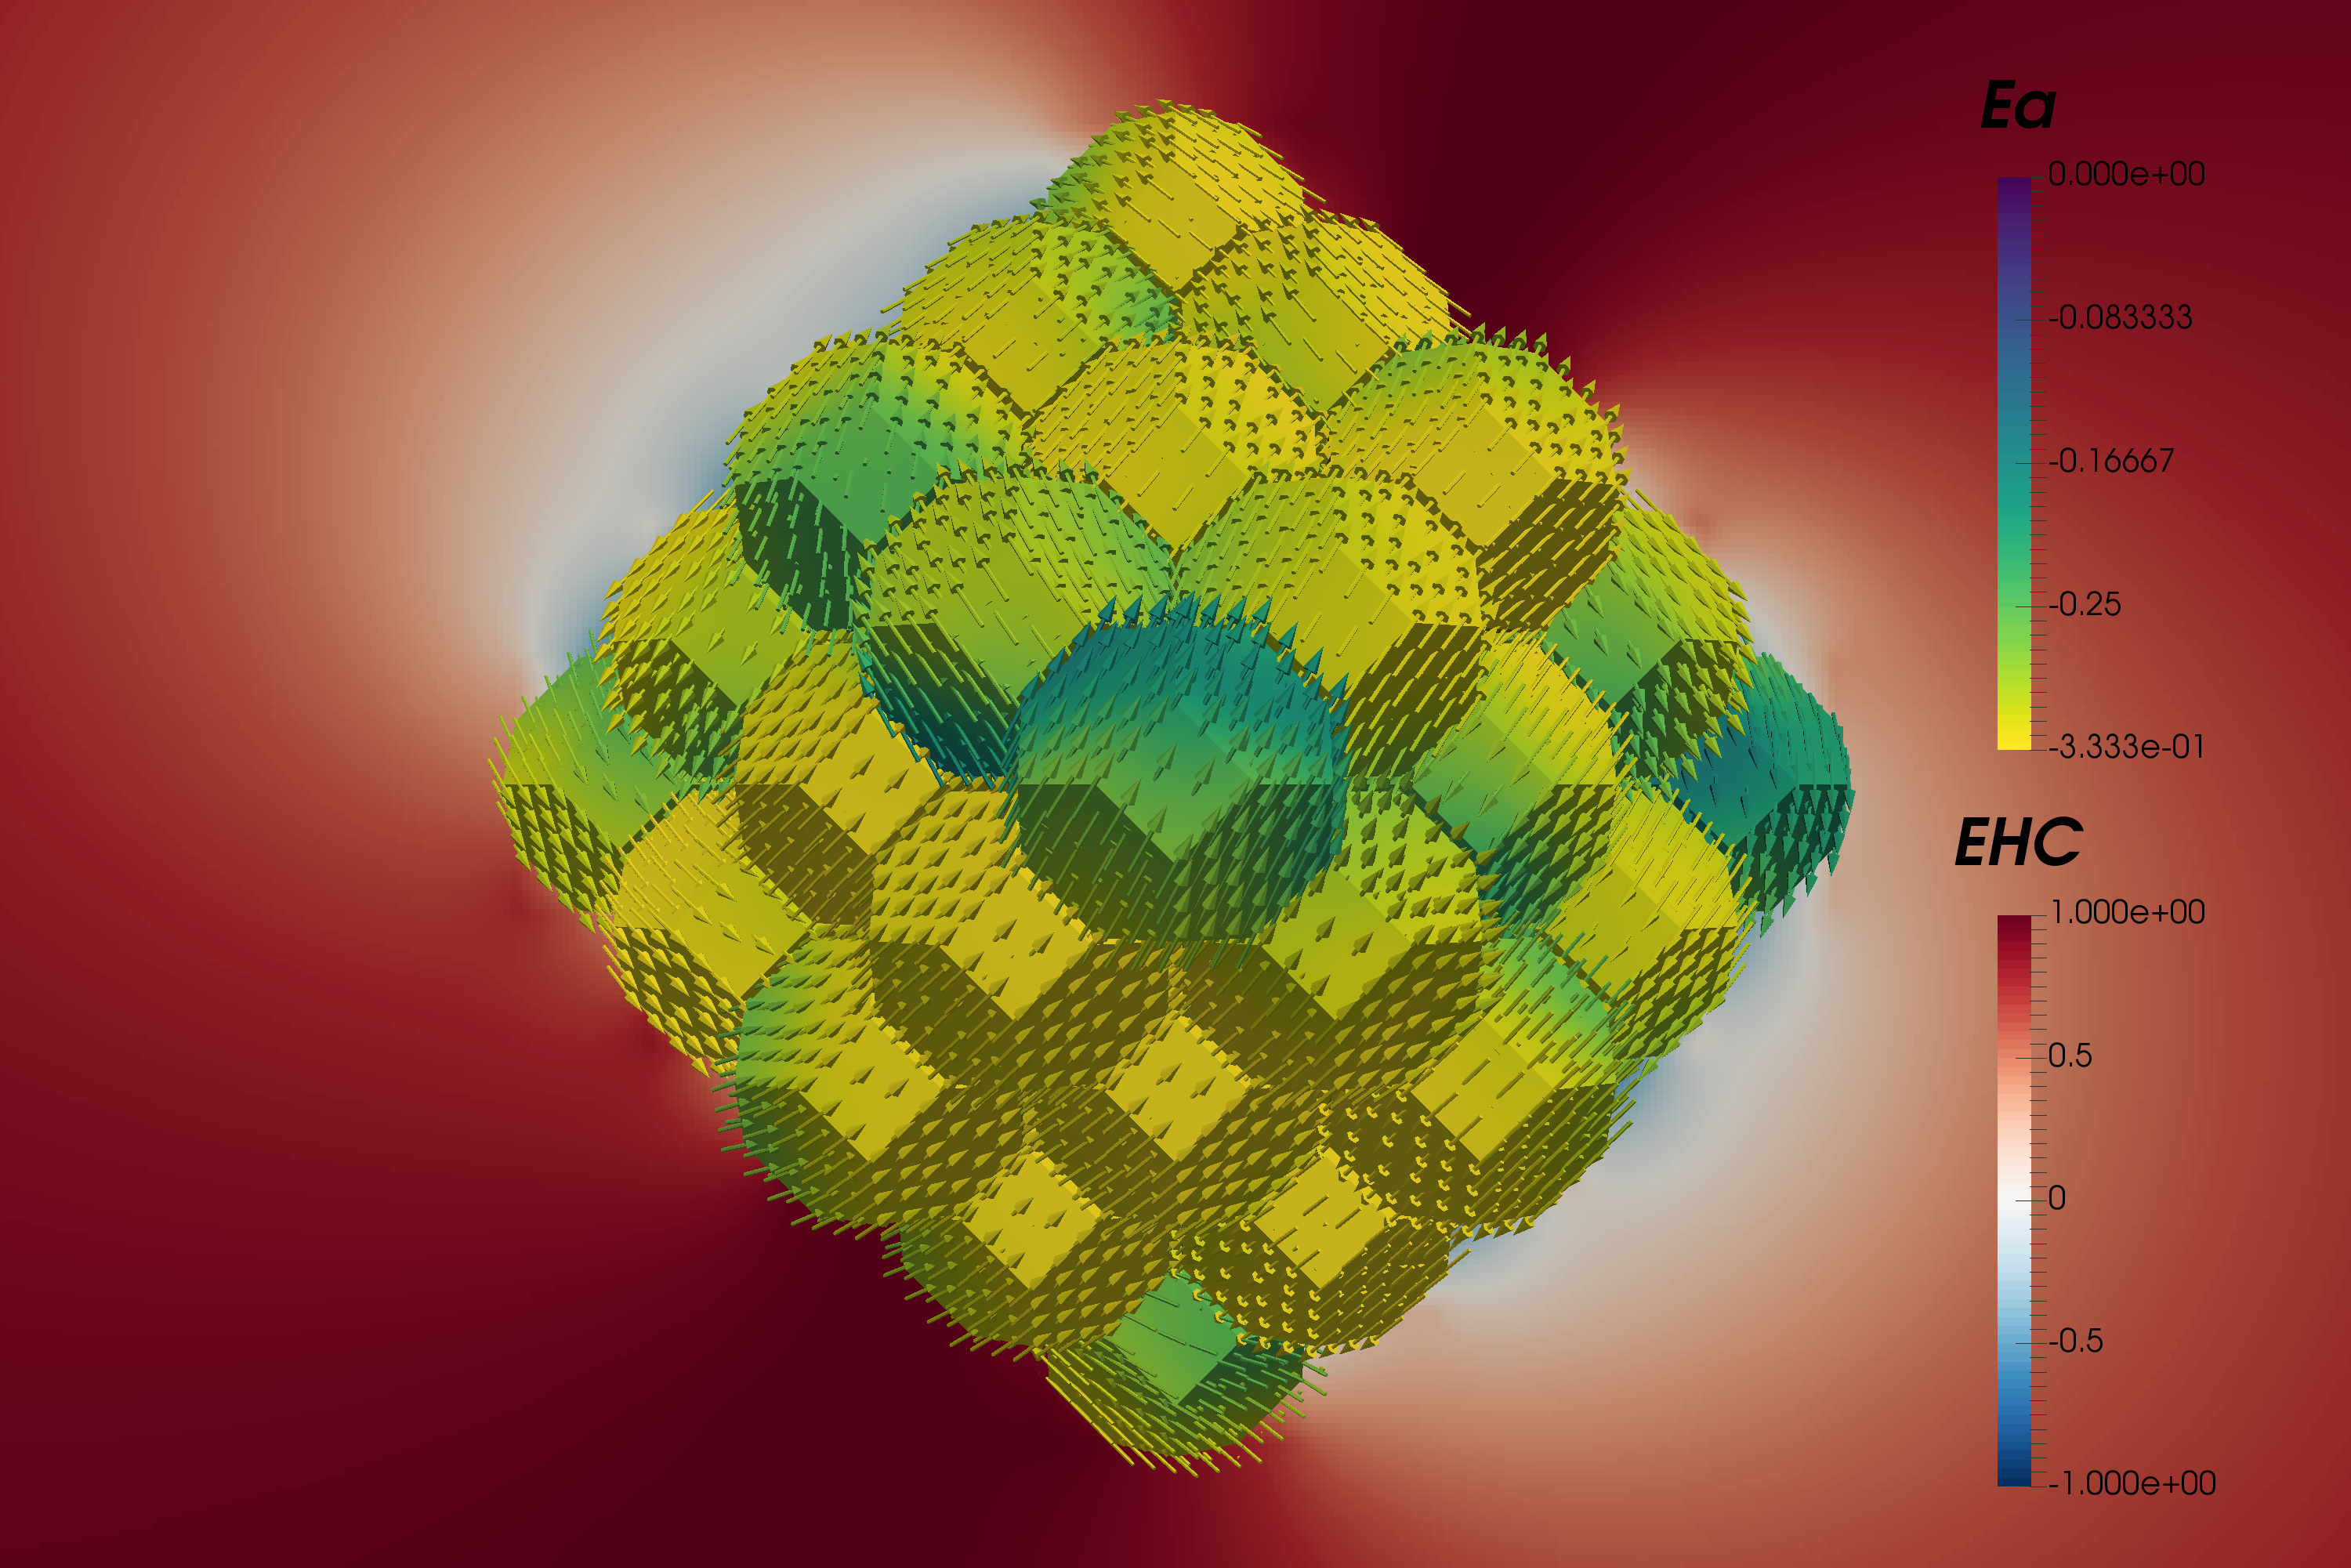
\includegraphics[width=\textwidth]{research-4/figs/fram_i21_f0_-z.png}
%\caption[Remanent state when the field is along an easy axis (view from +Z)]{Remanent state when the field is along an easy axis (view from +Z).}
%\label{FIG_15}
%\end{figure}
%
%\begin{figure}
%\centering
%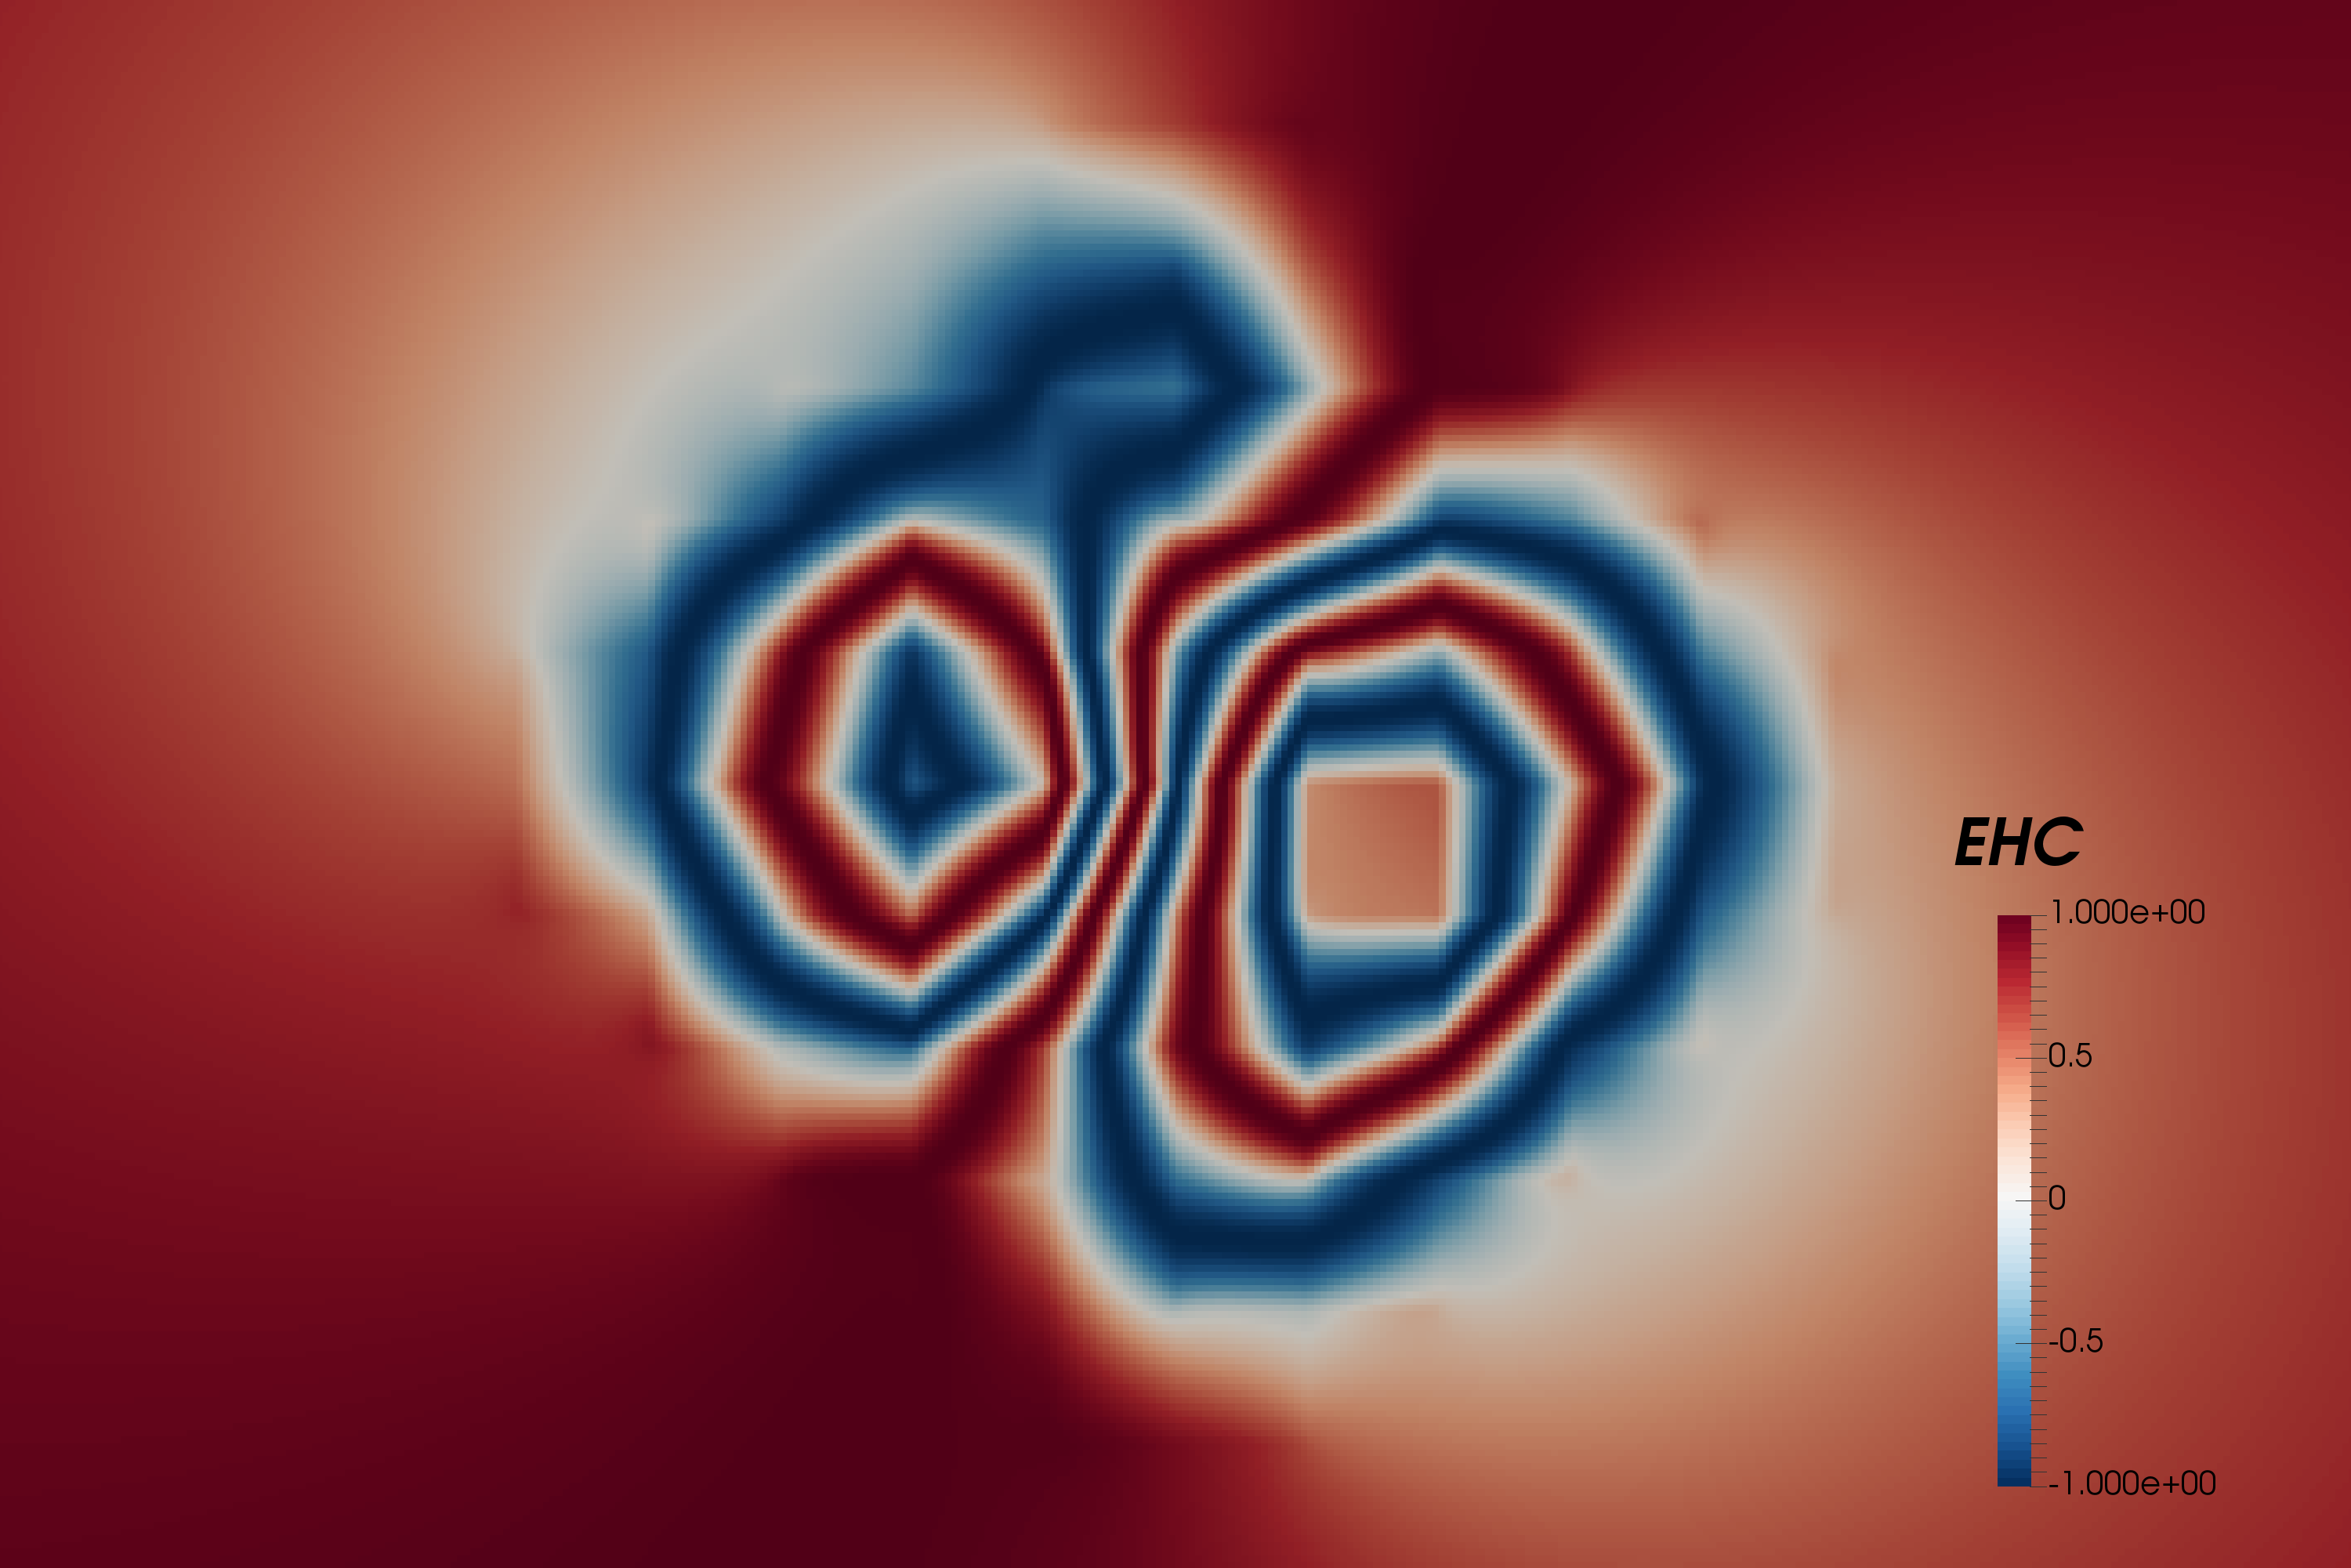
\includegraphics[width=\textwidth]{research-4/figs/fram_i21_f0_-z_EHC.png}
%\caption[Electron holography map of the remanent state when the field is along an easy axis (view from +Z)]{Electron holography map of the remanent state when the field is along an easy axis (view from +Z).}
%\label{FIG_16}
%\end{figure}
%
%\begin{figure}
%\centering
%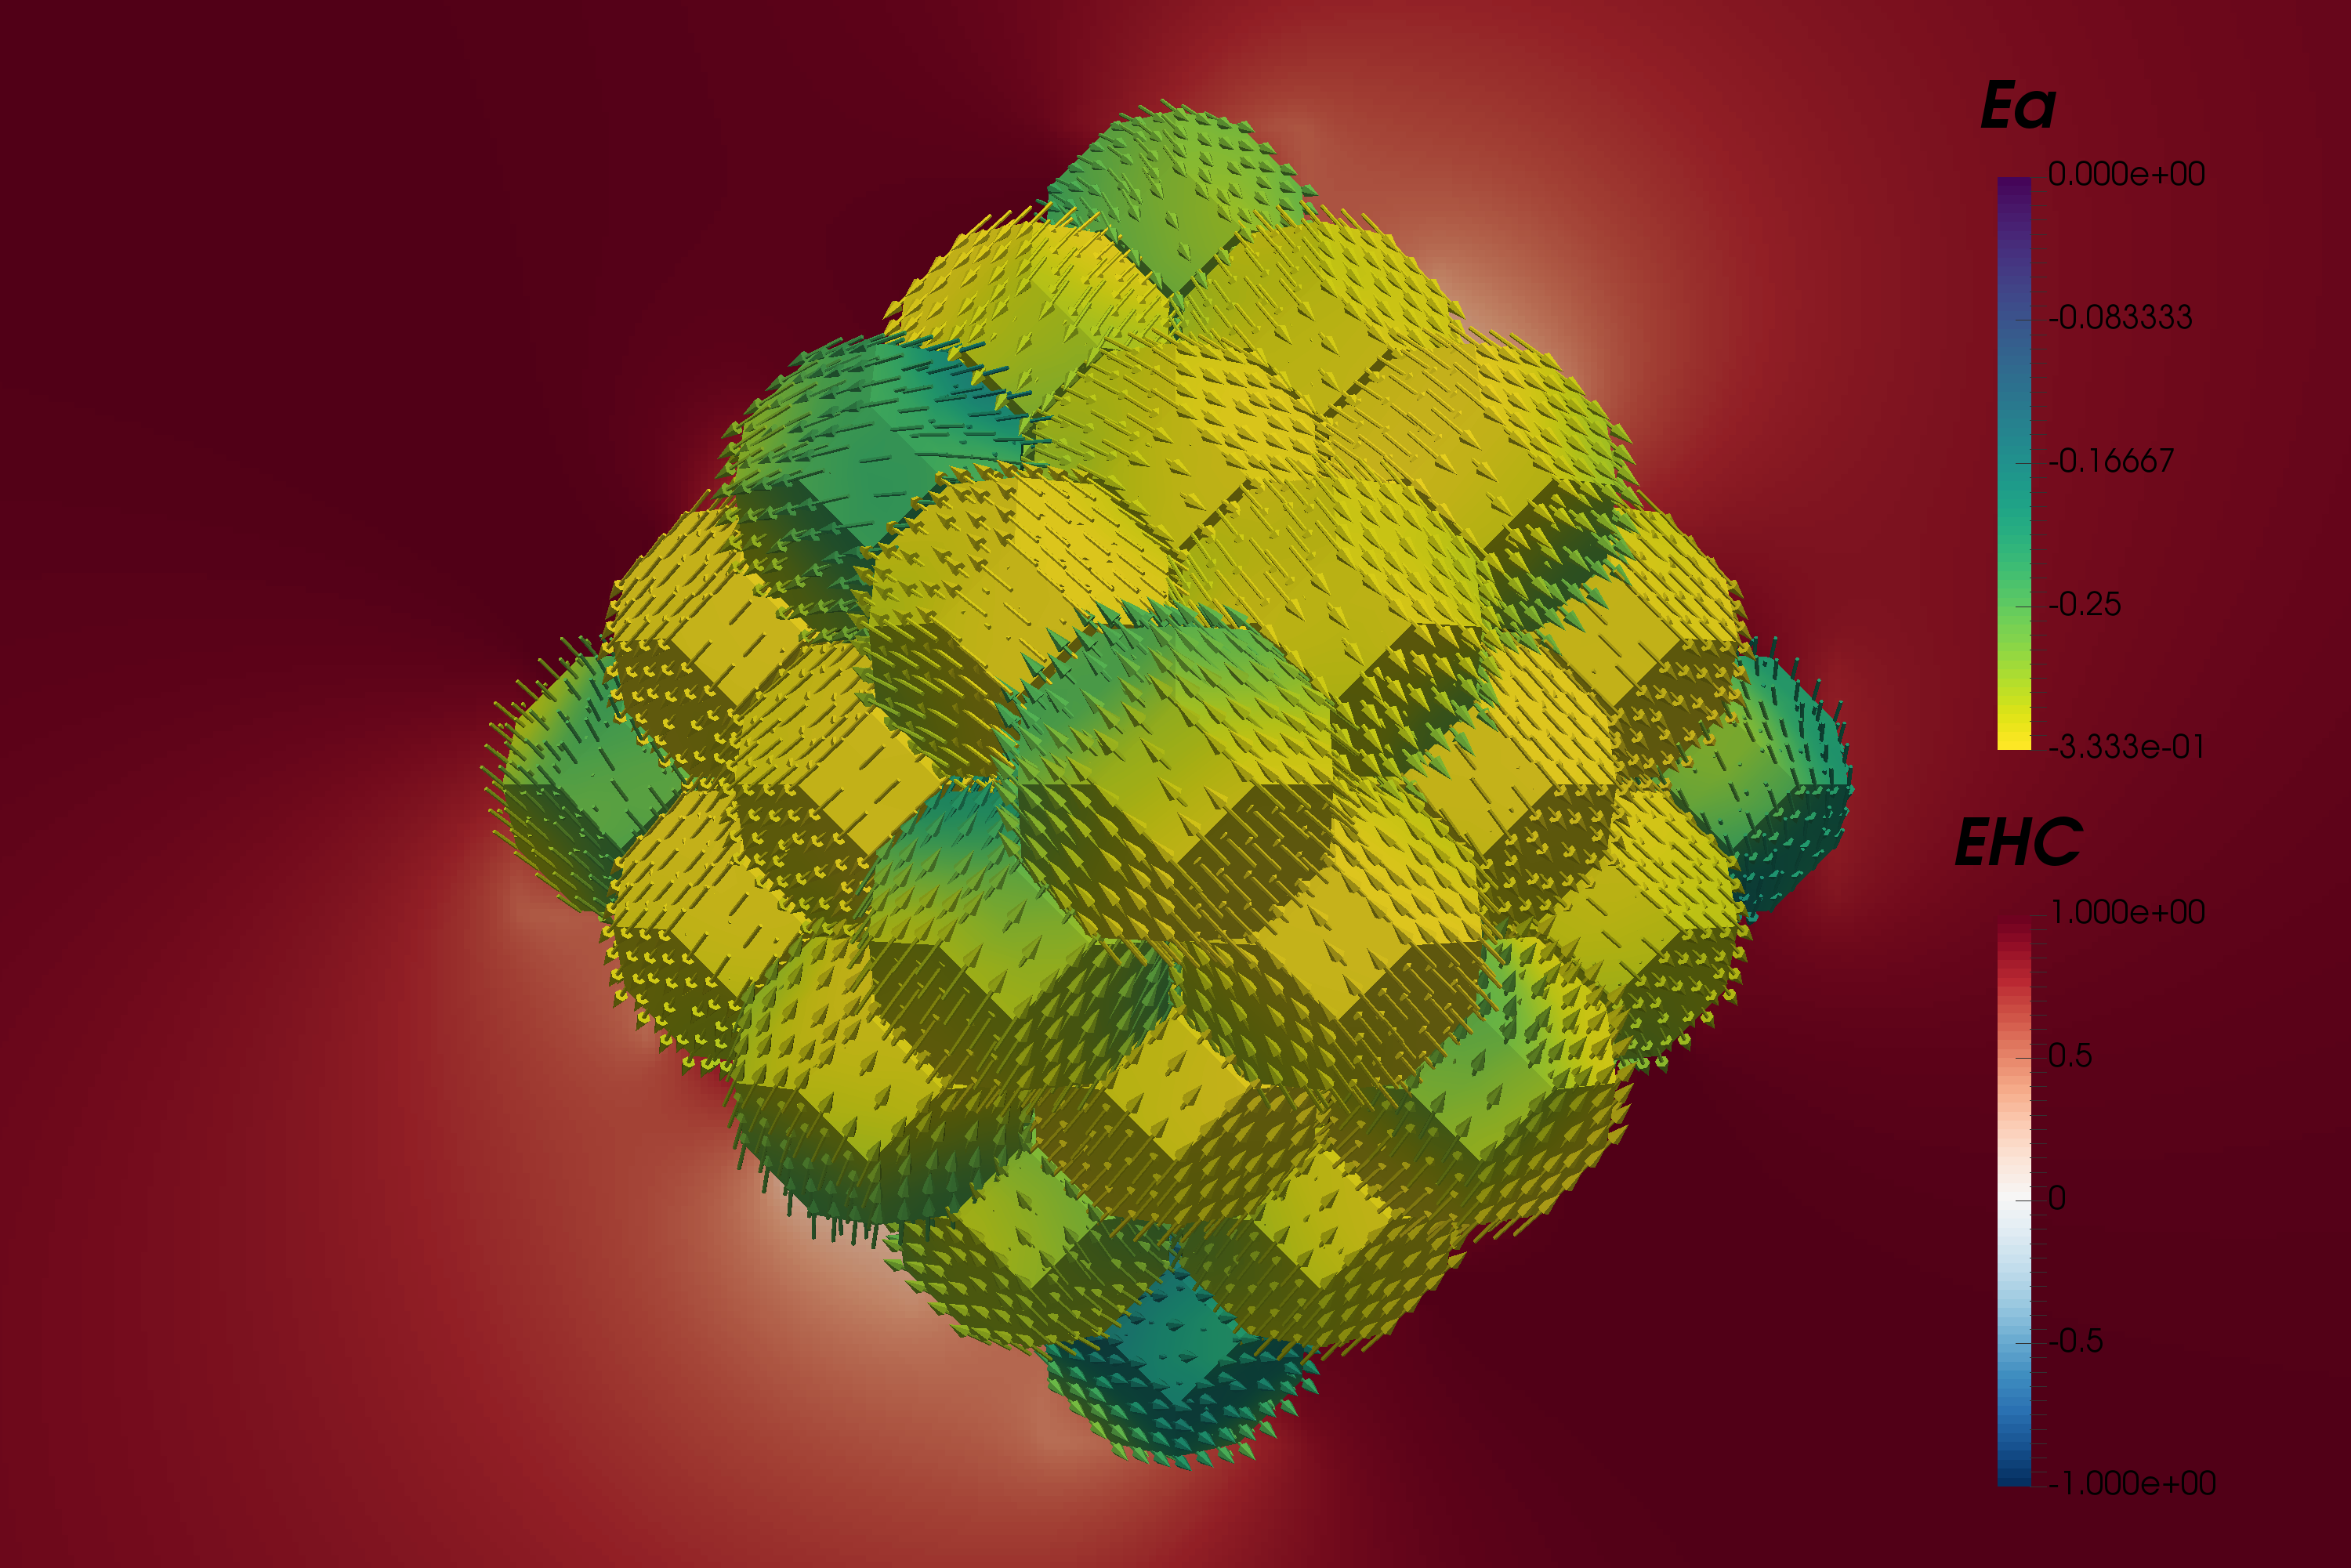
\includegraphics[width=\textwidth]{research-4/figs/fram_i21_f0_-y.png}
%\caption[Remanent state when the field is along an easy axis (view from +Y)]{Remanent state when the field is along an easy axis (view from +Y).}
%\label{FIG_17}
%\end{figure}
%
%\begin{figure}
%\centering
%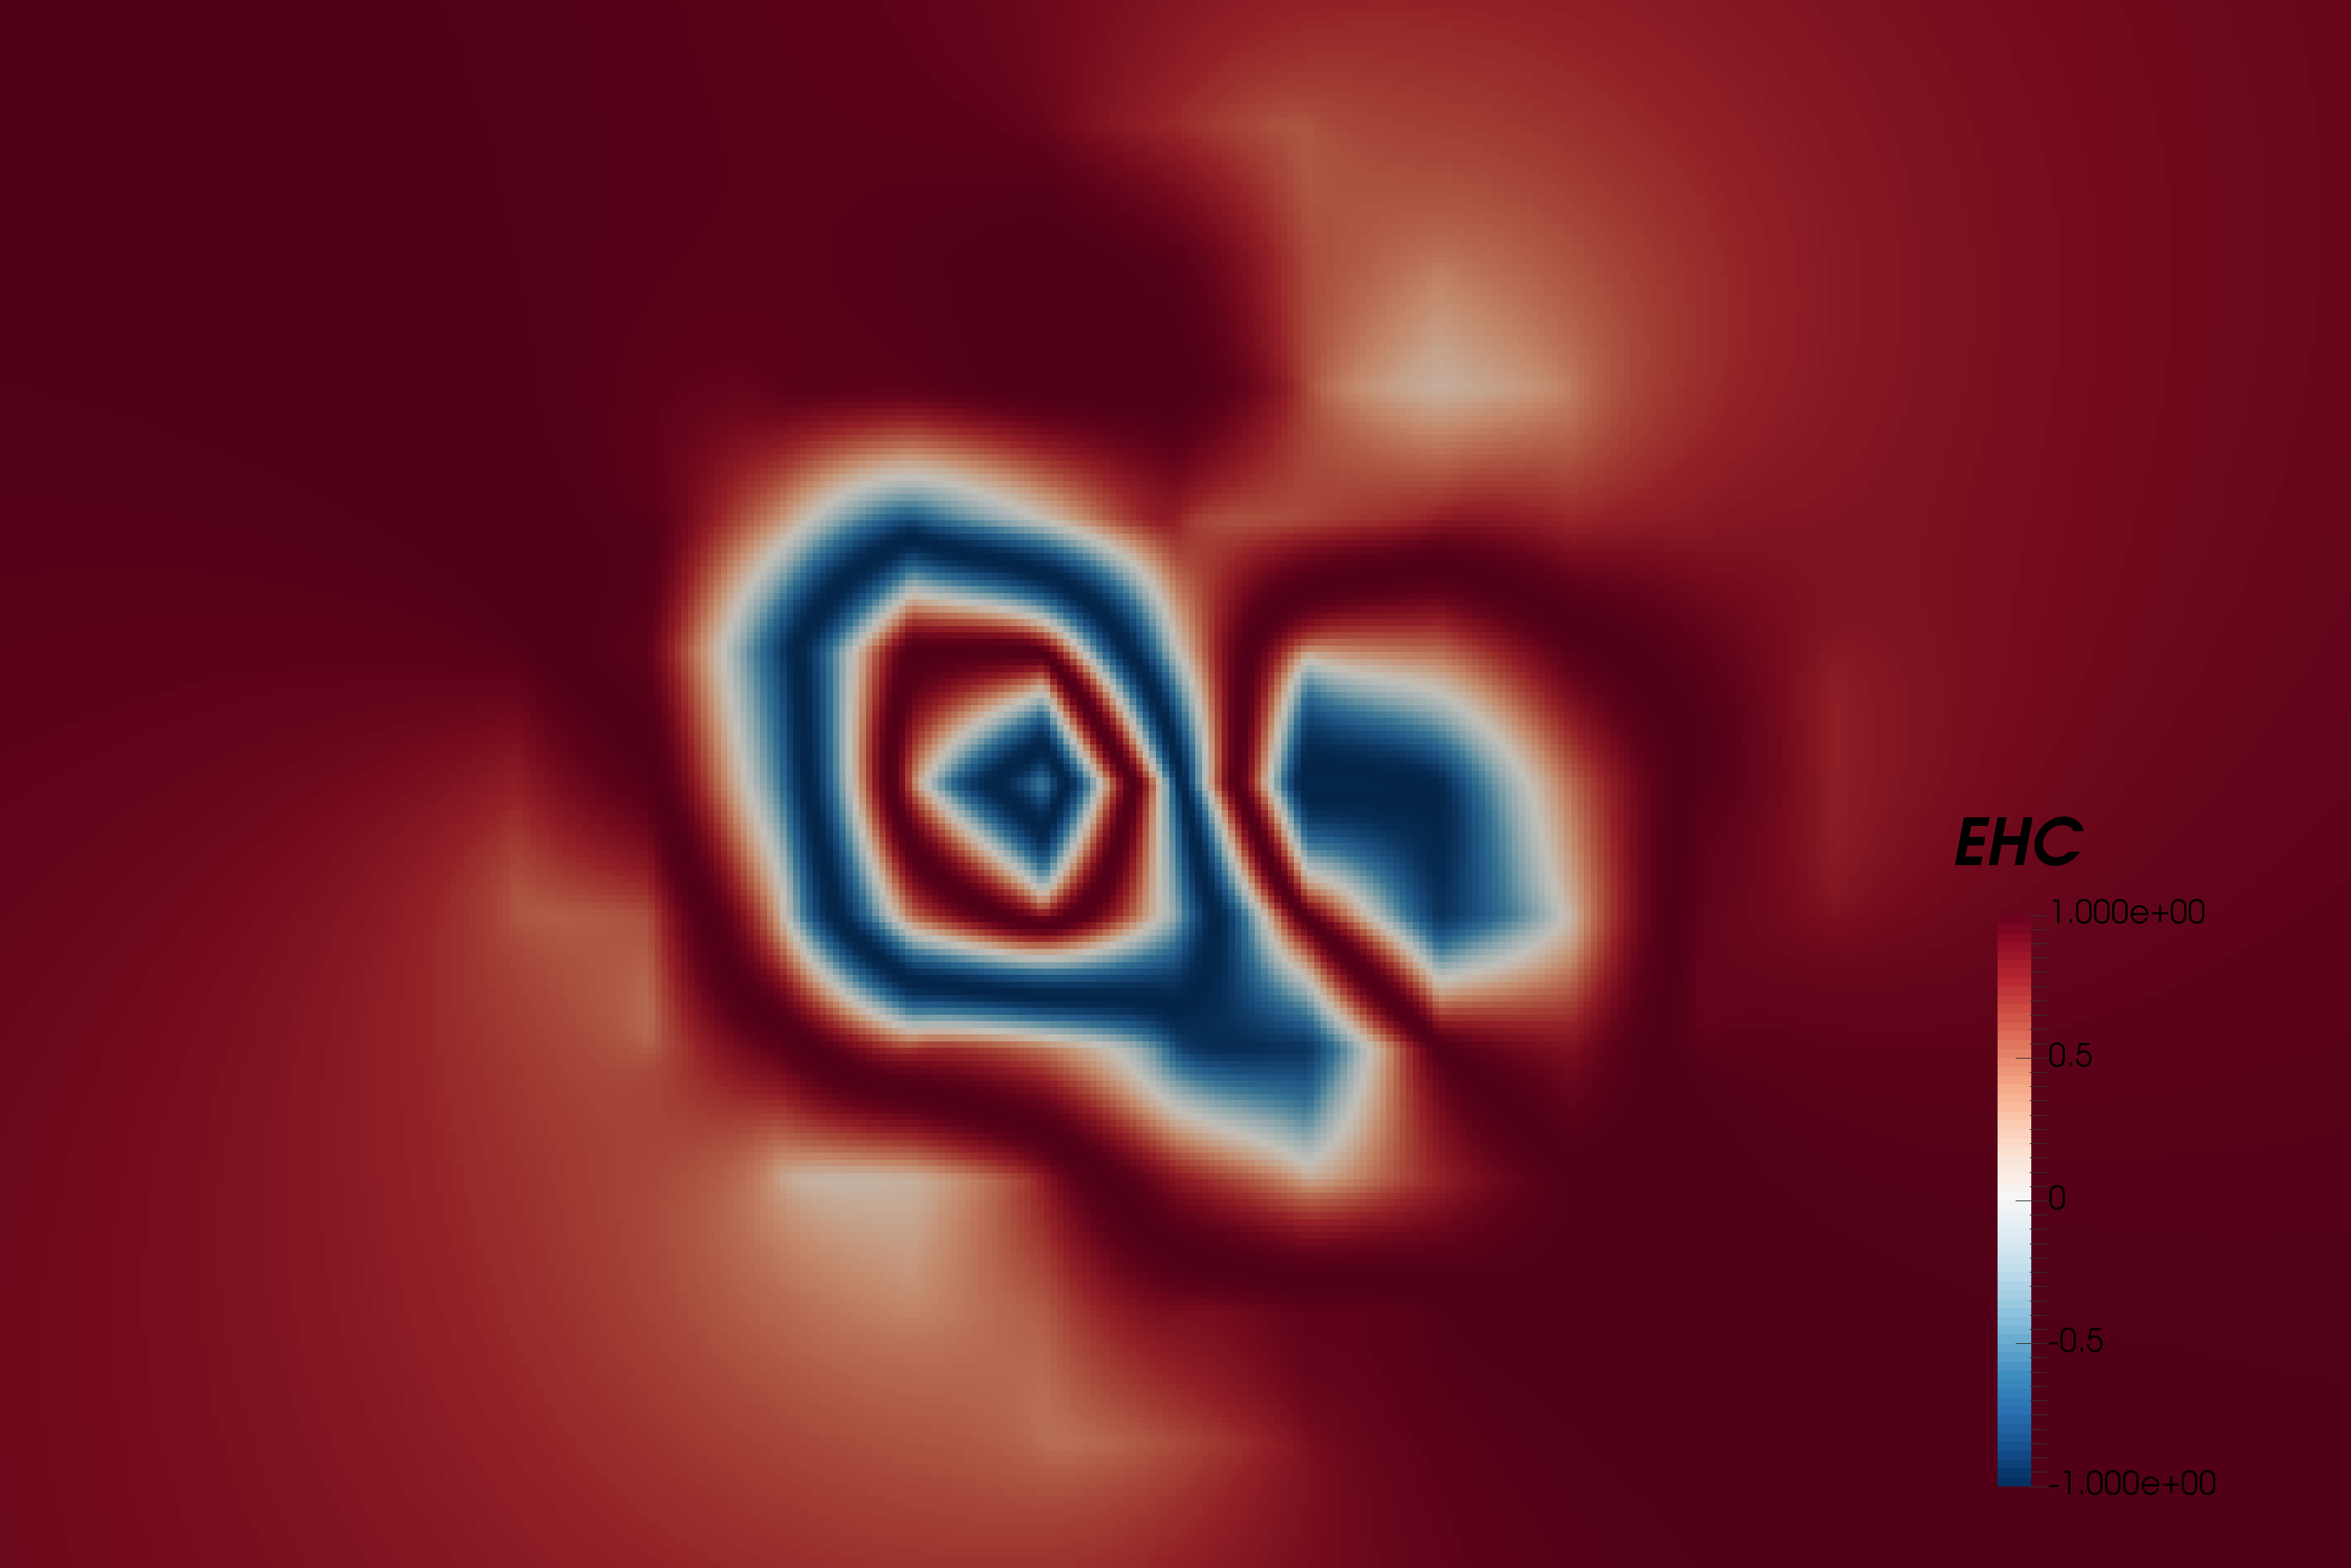
\includegraphics[width=\textwidth]{research-4/figs/fram_i21_f0_-y_EHC.png}
%\caption[Electron holography map of the remanent state when the field is along an easy axis (view from +Y)]{Electron holography map of the remanent state when the field is along an easy axis (view from +Y).}
%\label{FIG_18}
%\end{figure}
%
%\begin{figure}
%\centering
%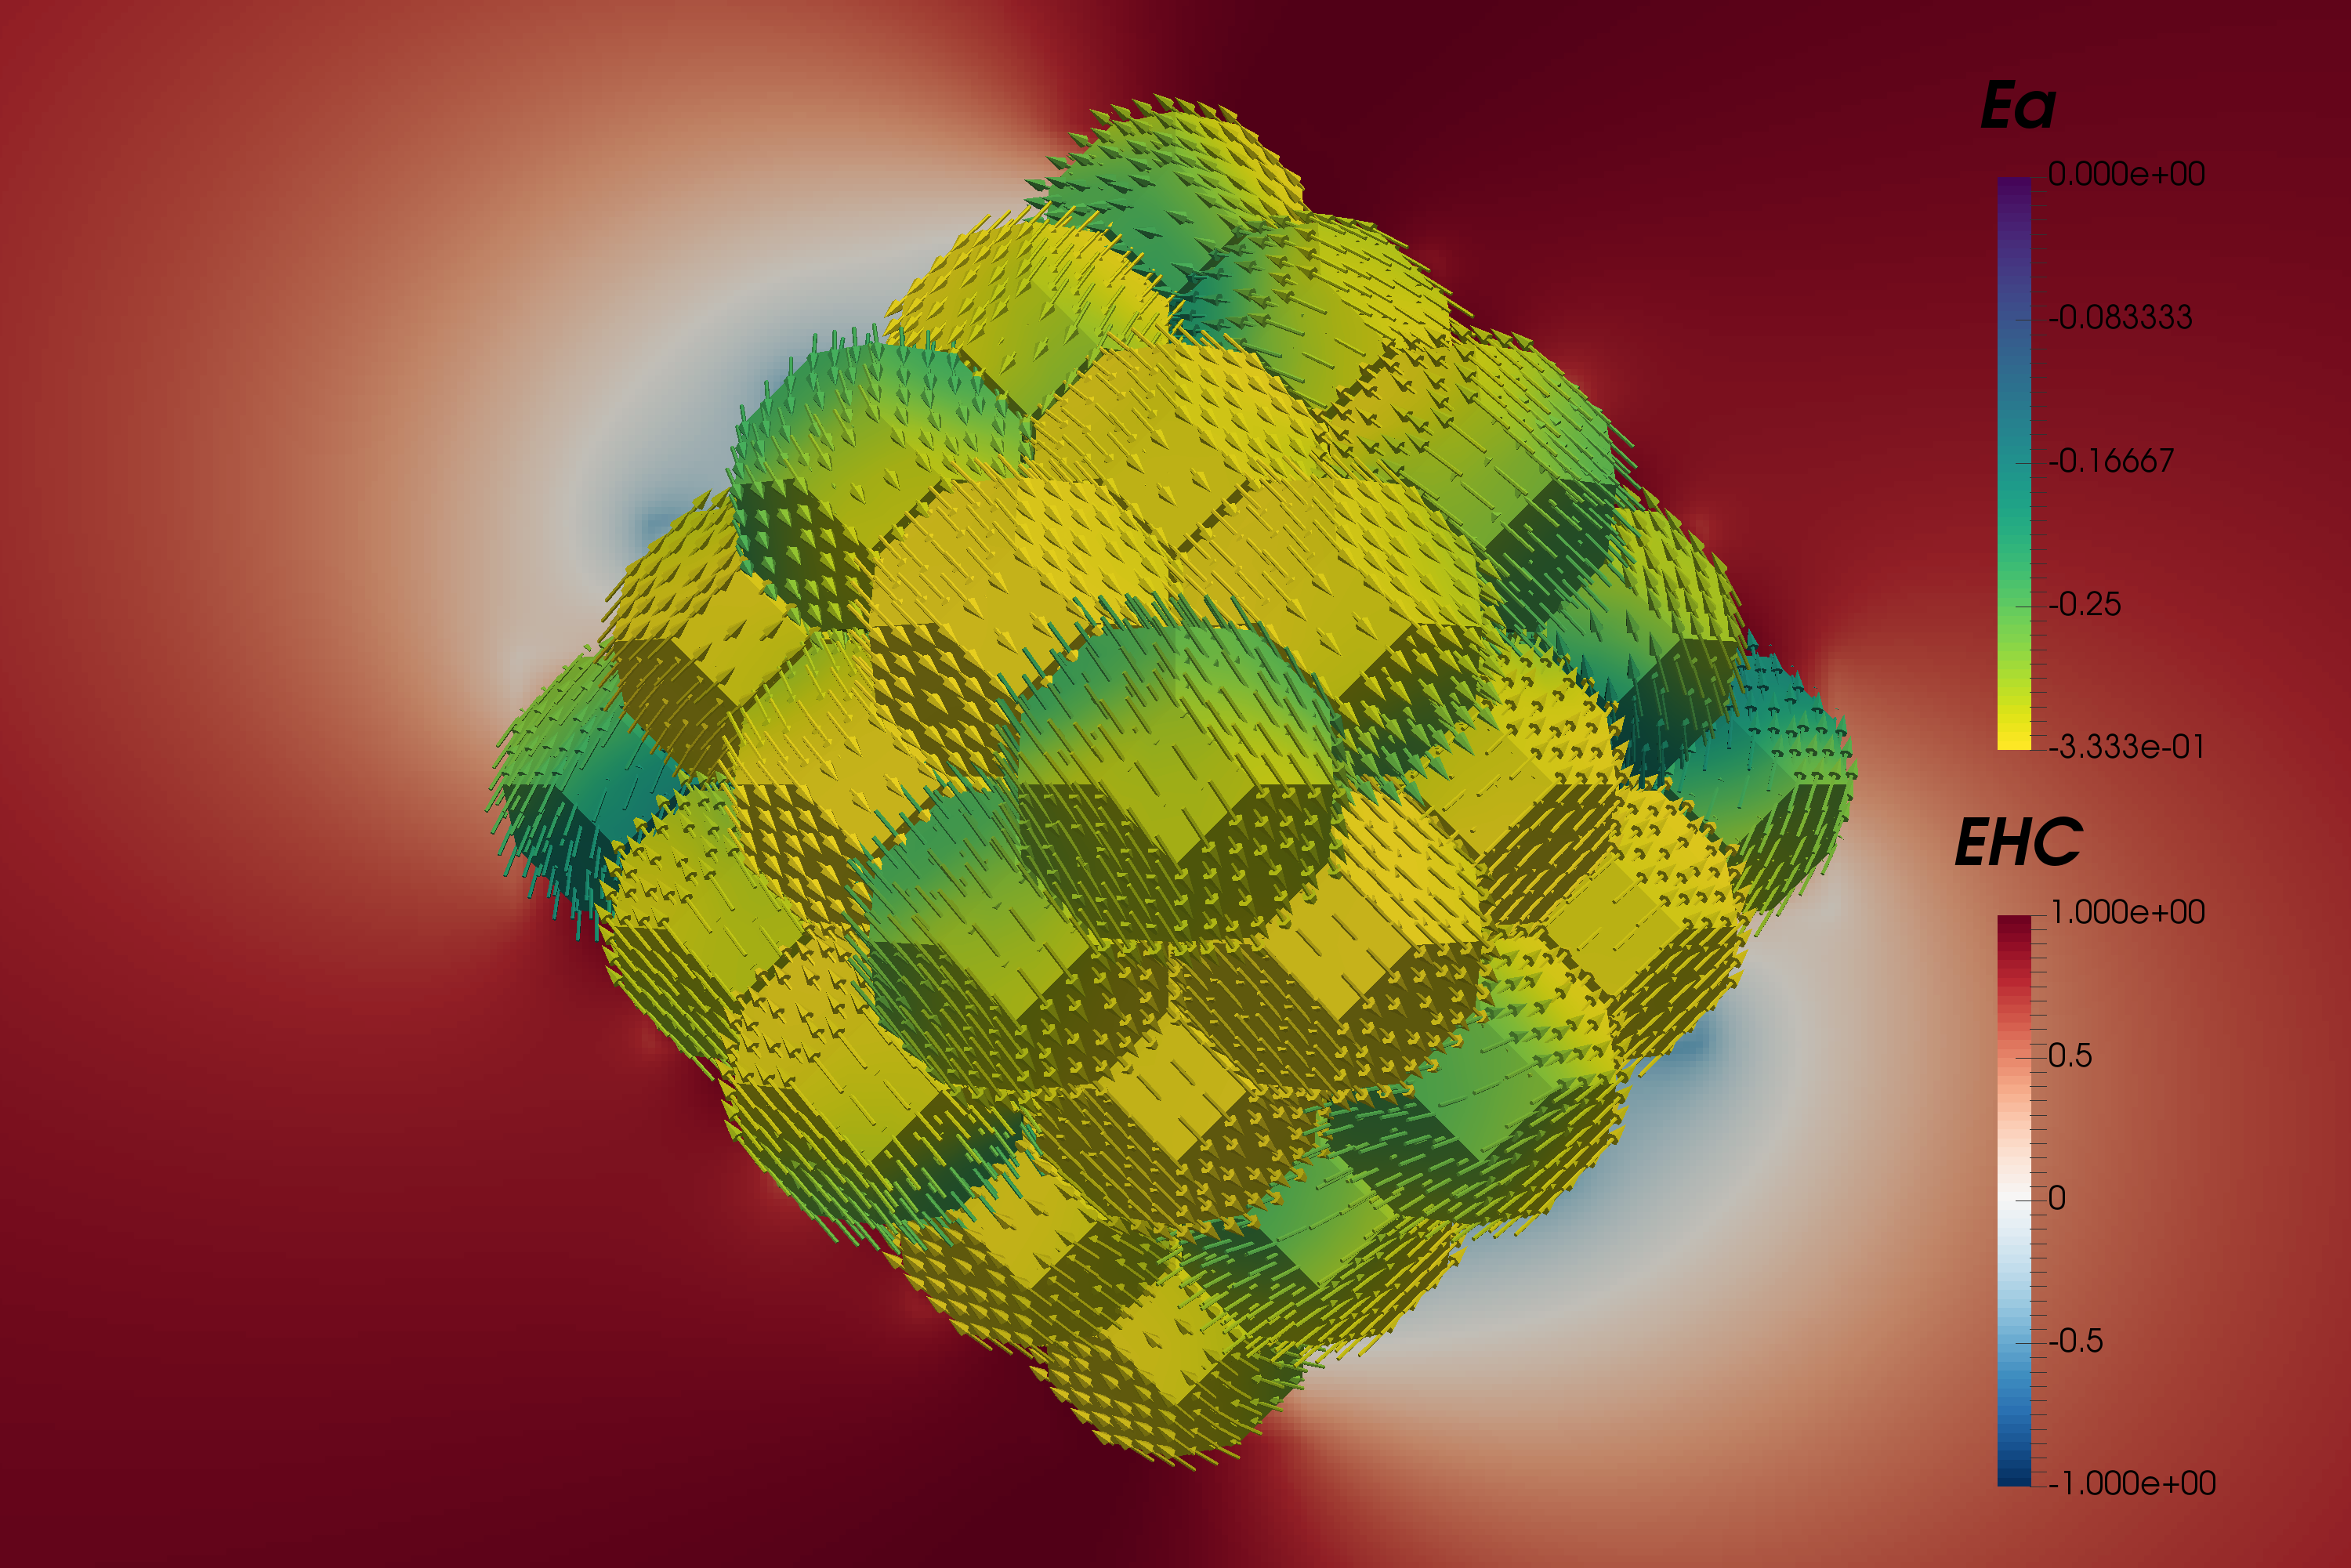
\includegraphics[width=\textwidth]{research-4/figs/fram_i21_f0_-x.png}
%\caption[Remanent state when the field is along an easy axis (view from +X)]{Remanent state when the field is along an easy axis (view from +X).}
%\label{FIG_19}
%\end{figure}
%
%\begin{figure}
%\centering
%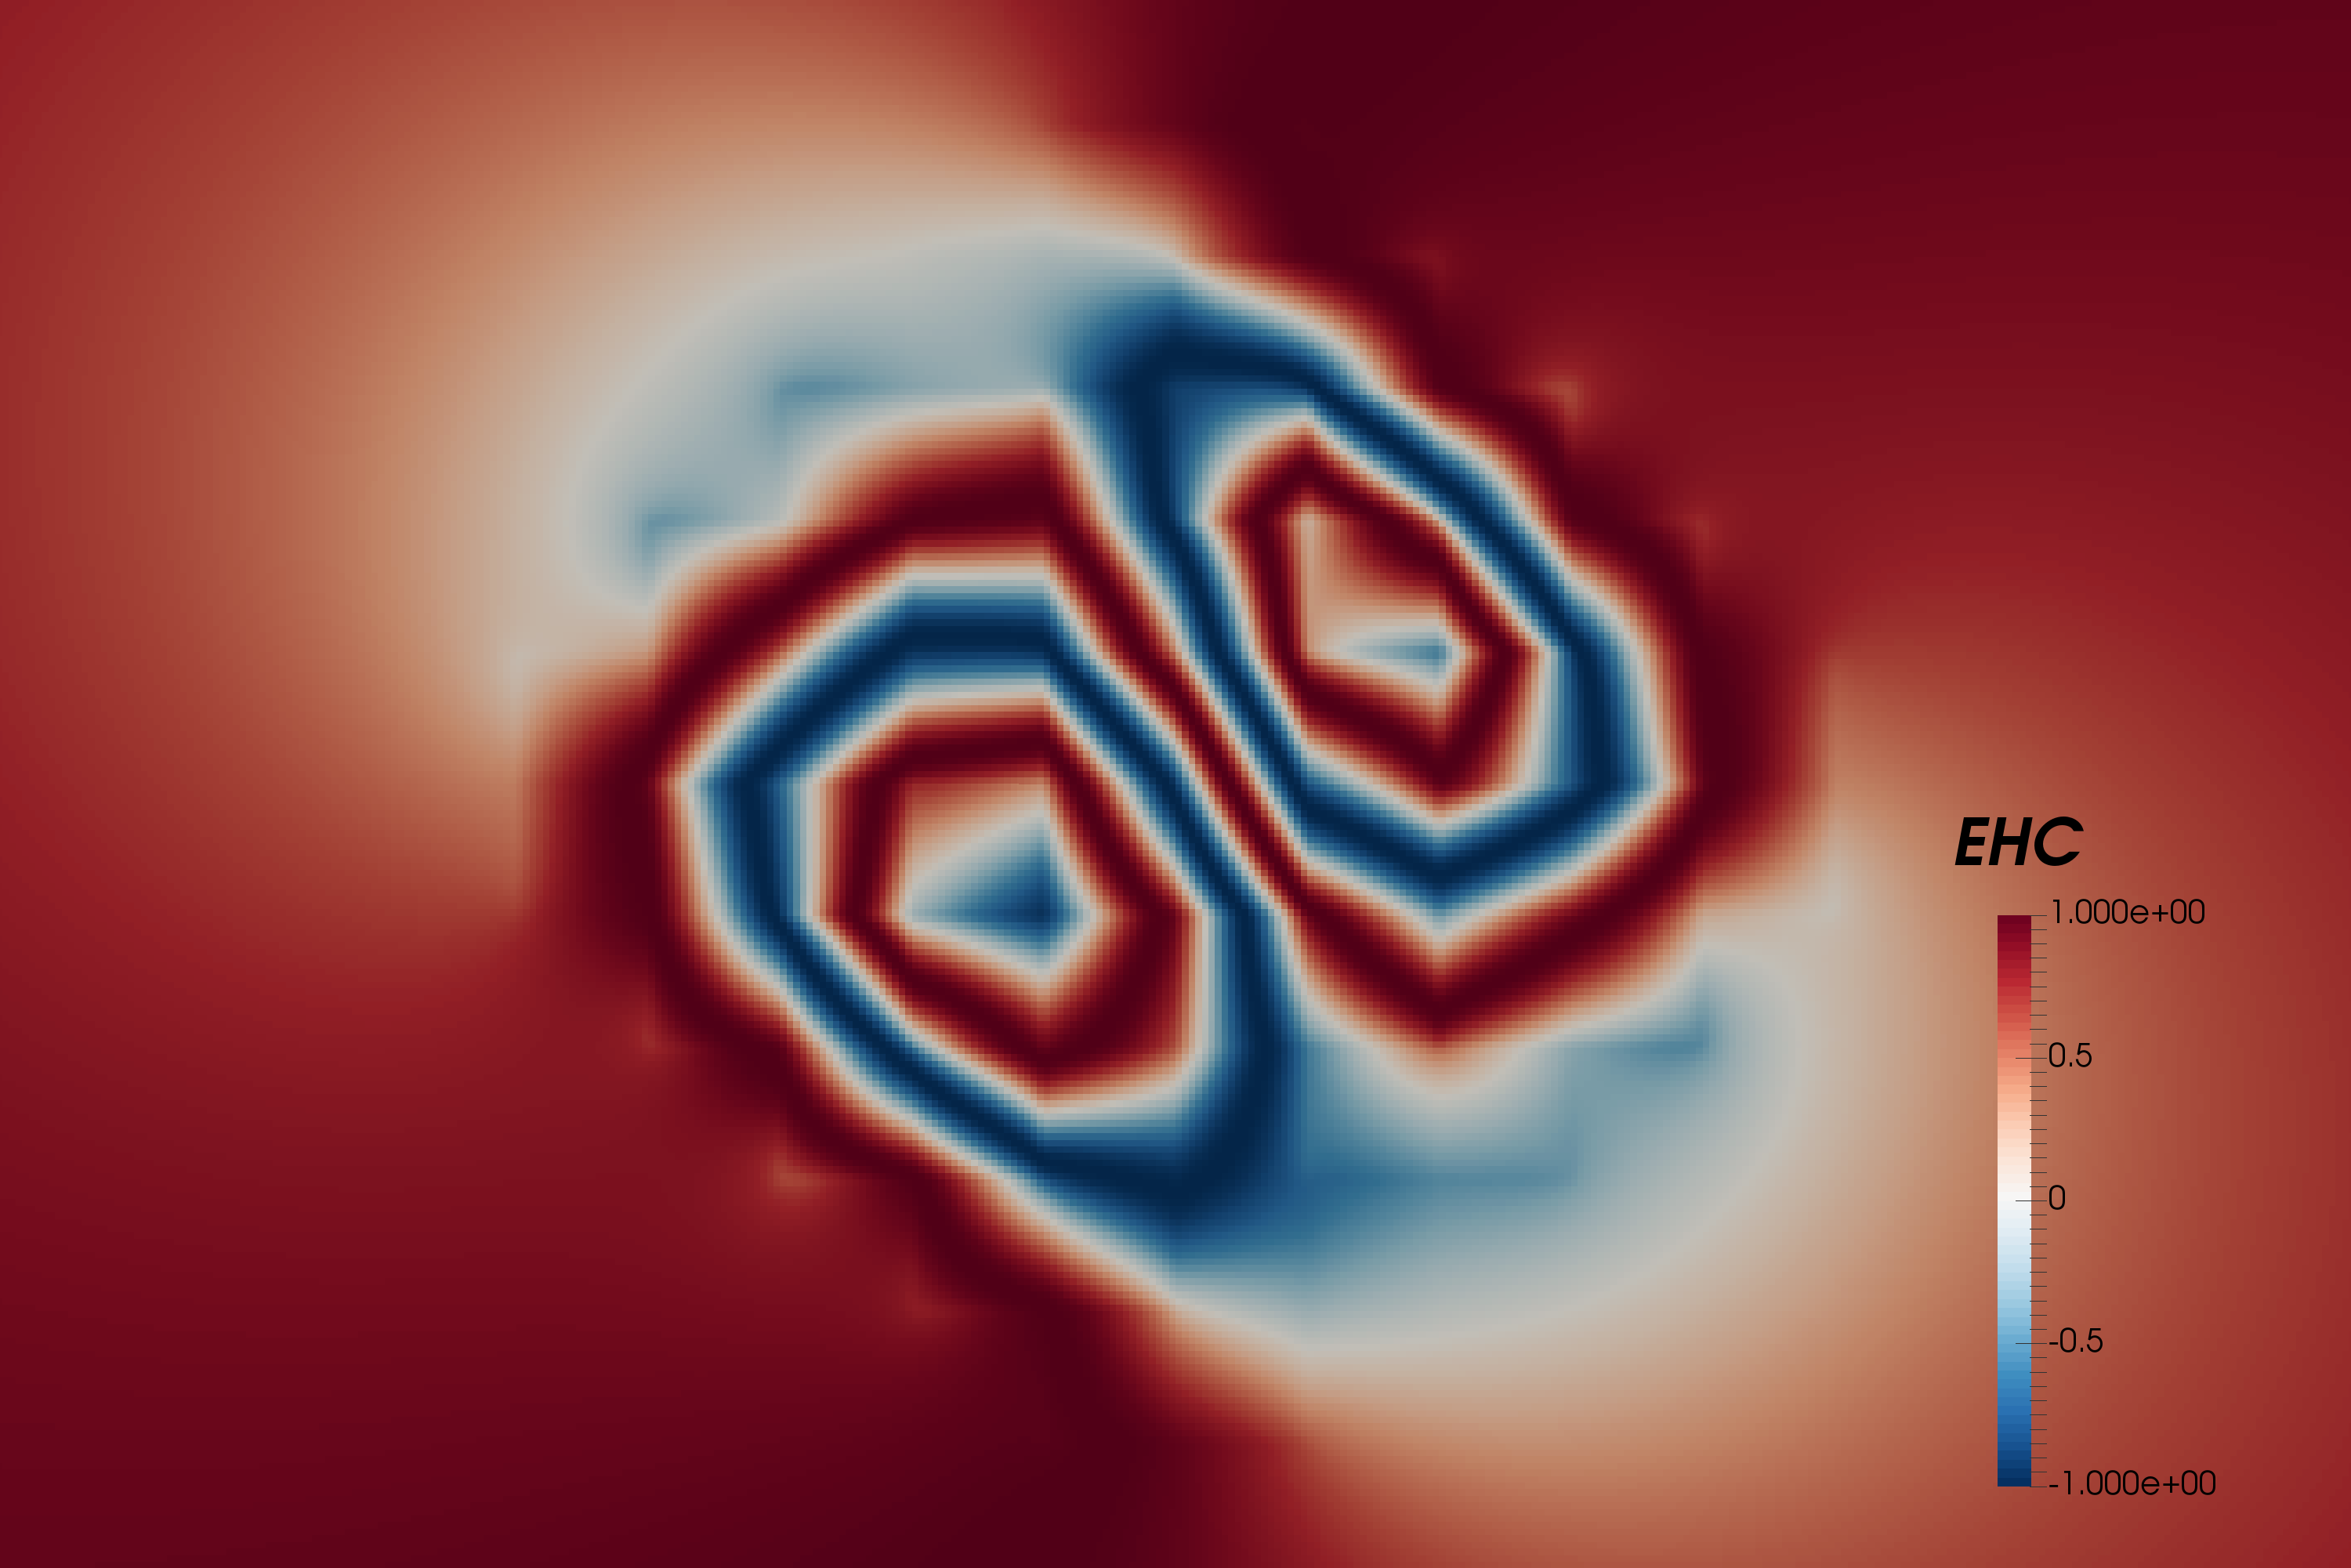
\includegraphics[width=\textwidth]{research-4/figs/fram_i21_f0_-x_EHC.png}
%\caption[Electron holography map of the remanent state when the field is along an easy axis (view from +X)]{Electron holography map of the remanent state when the field is along an easy axis (view from +X).}
%\label{FIG_20}
%\end{figure}
%
%\begin{figure}
%\centering
%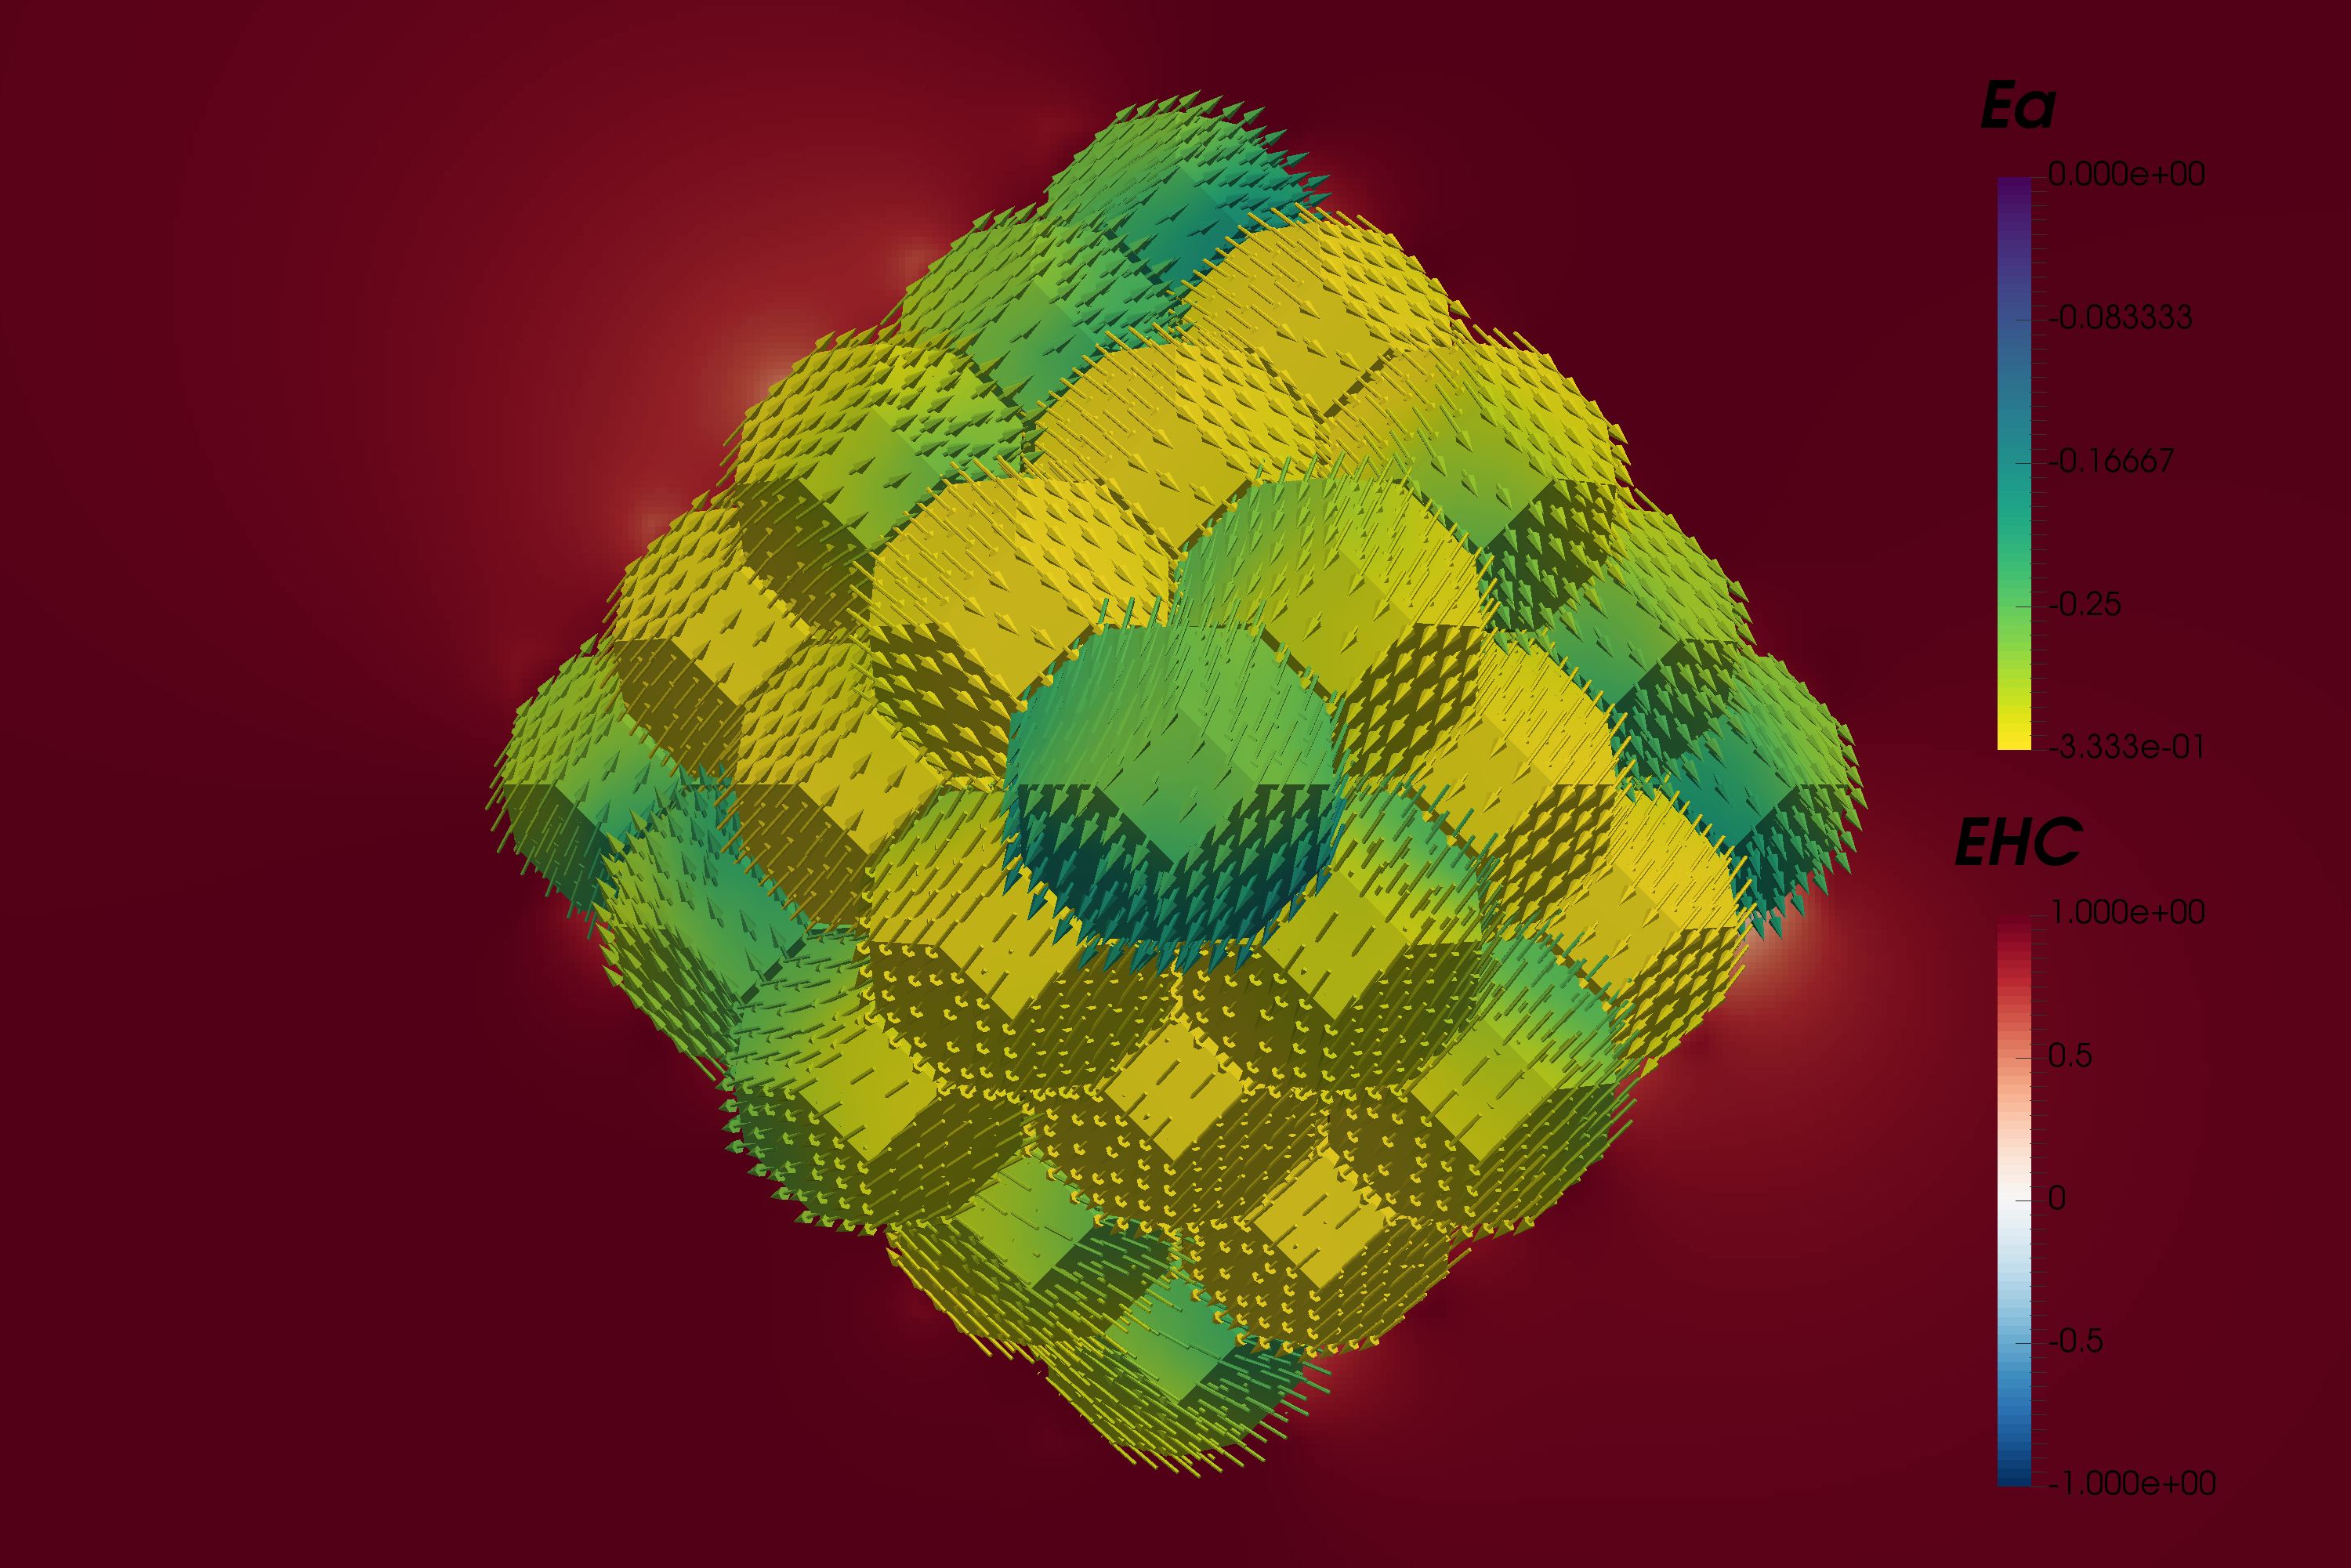
\includegraphics[width=\textwidth]{research-4/figs/fram_i16_f0_-z.png}
%\caption[Remanent state when the field is along a hard axis (view from +Z)]{Remanent state when the field is along a hard axis (view from +Z).}
%\label{FIG_21}
%\end{figure}
%
%\begin{figure}
%\centering
%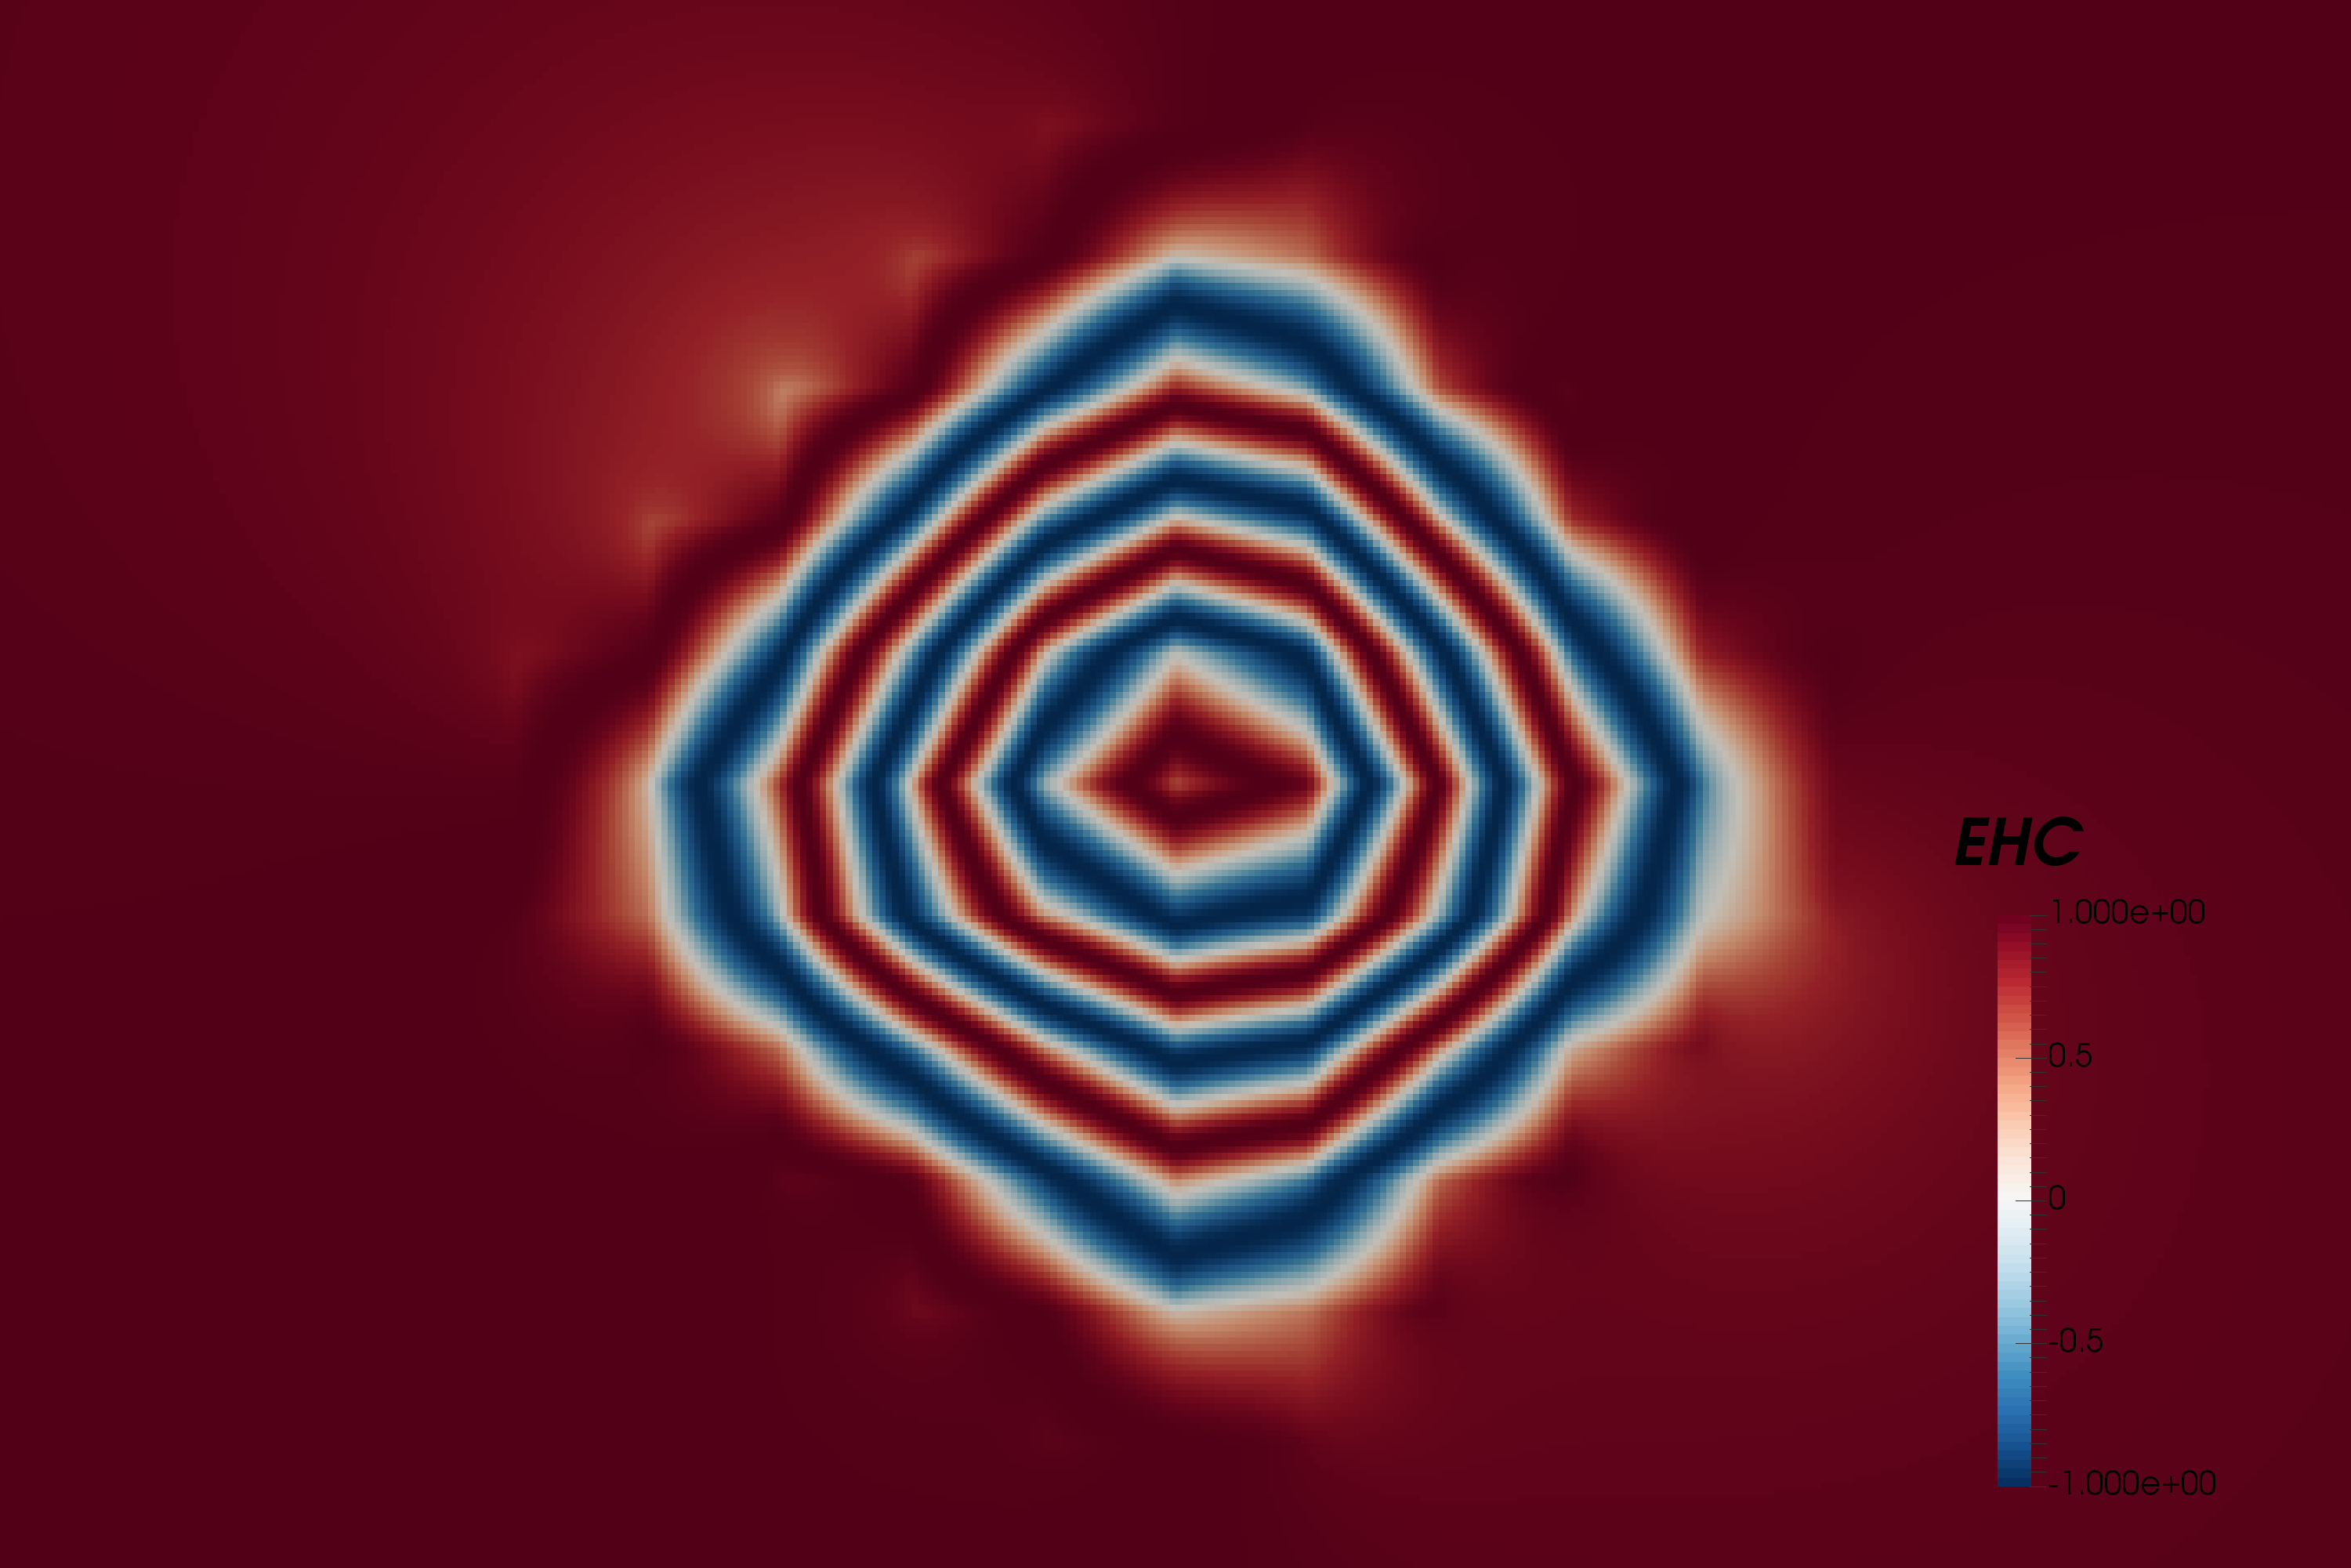
\includegraphics[width=\textwidth]{research-4/figs/fram_i16_f0_-z_EHC.png}
%\caption[Electron holography map of the remanent state when the field is along a hard axis (view from +Z)]{Electron holography map of the remanent state when the field is along a hard axis (view from +Z).}
%\label{FIG_22}
%\end{figure}
%
%\begin{figure}
%\centering
%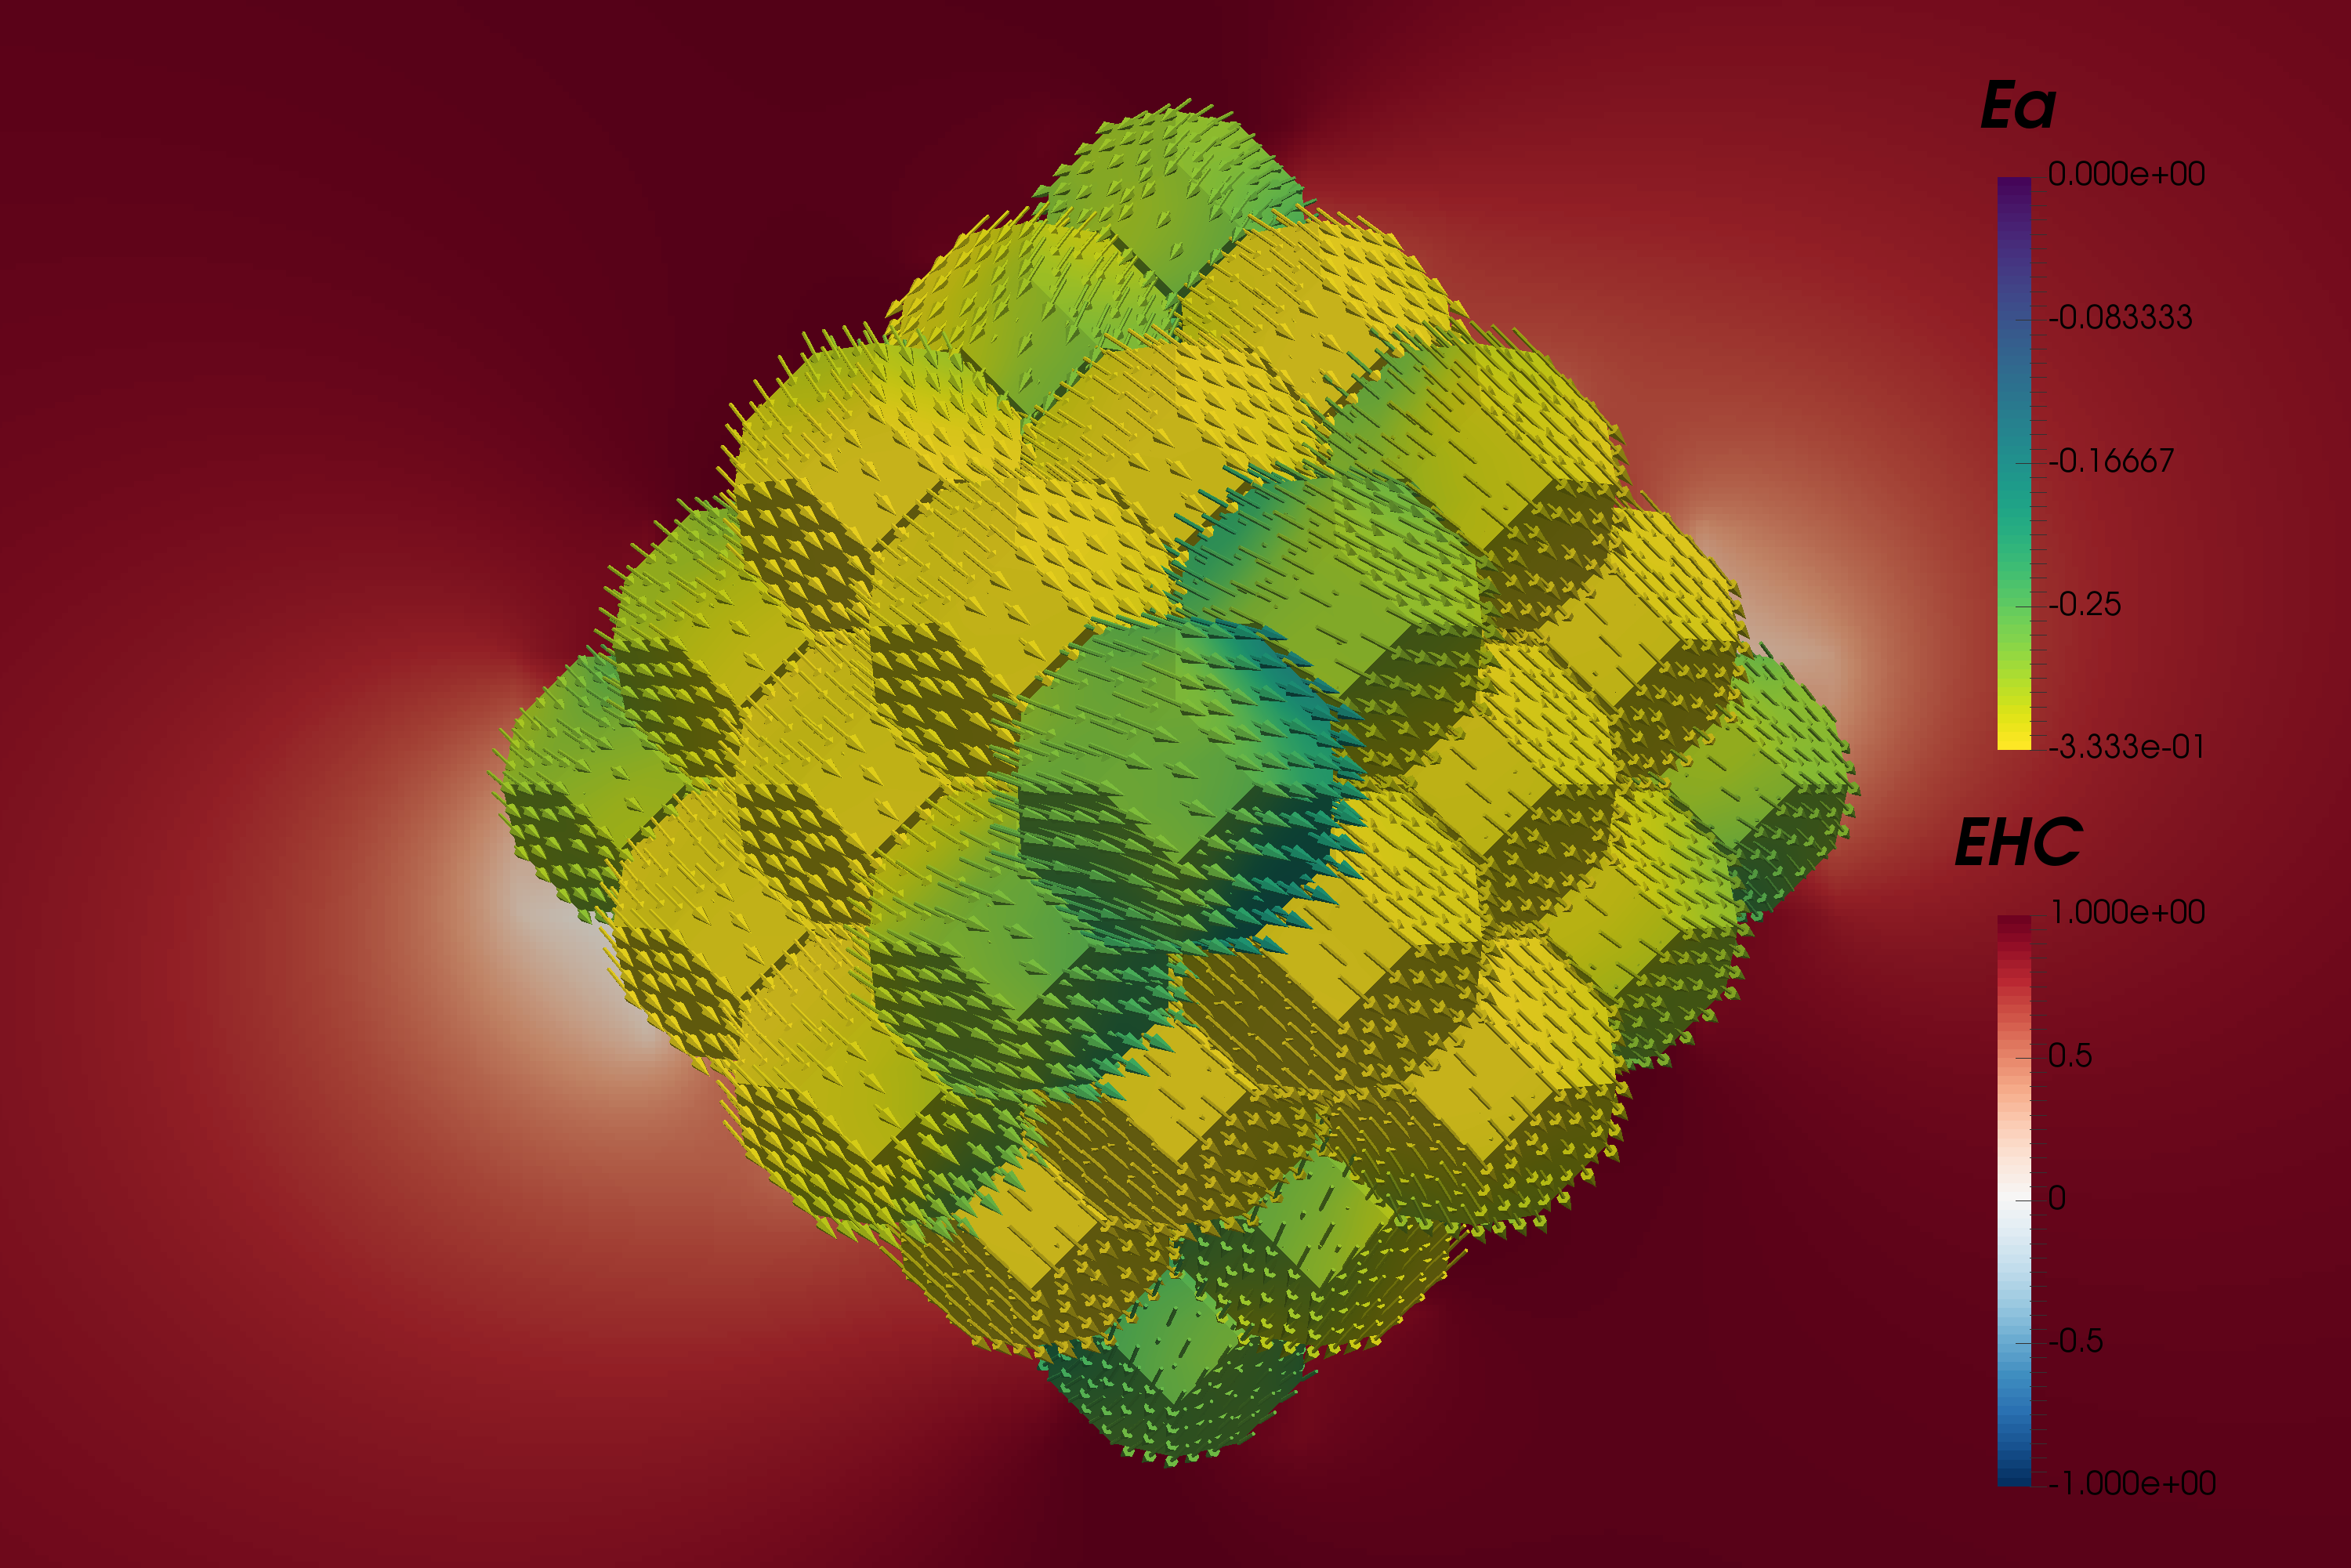
\includegraphics[width=\textwidth]{research-4/figs/fram_i16_f0_-y.png}
%\caption[Remanent state when the field is along a hard axis (view from +Y)]{Remanent state when the field is along a hard axis (view from +Y).}
%\label{FIG_23}
%\end{figure}
%
%\begin{figure}
%\centering
%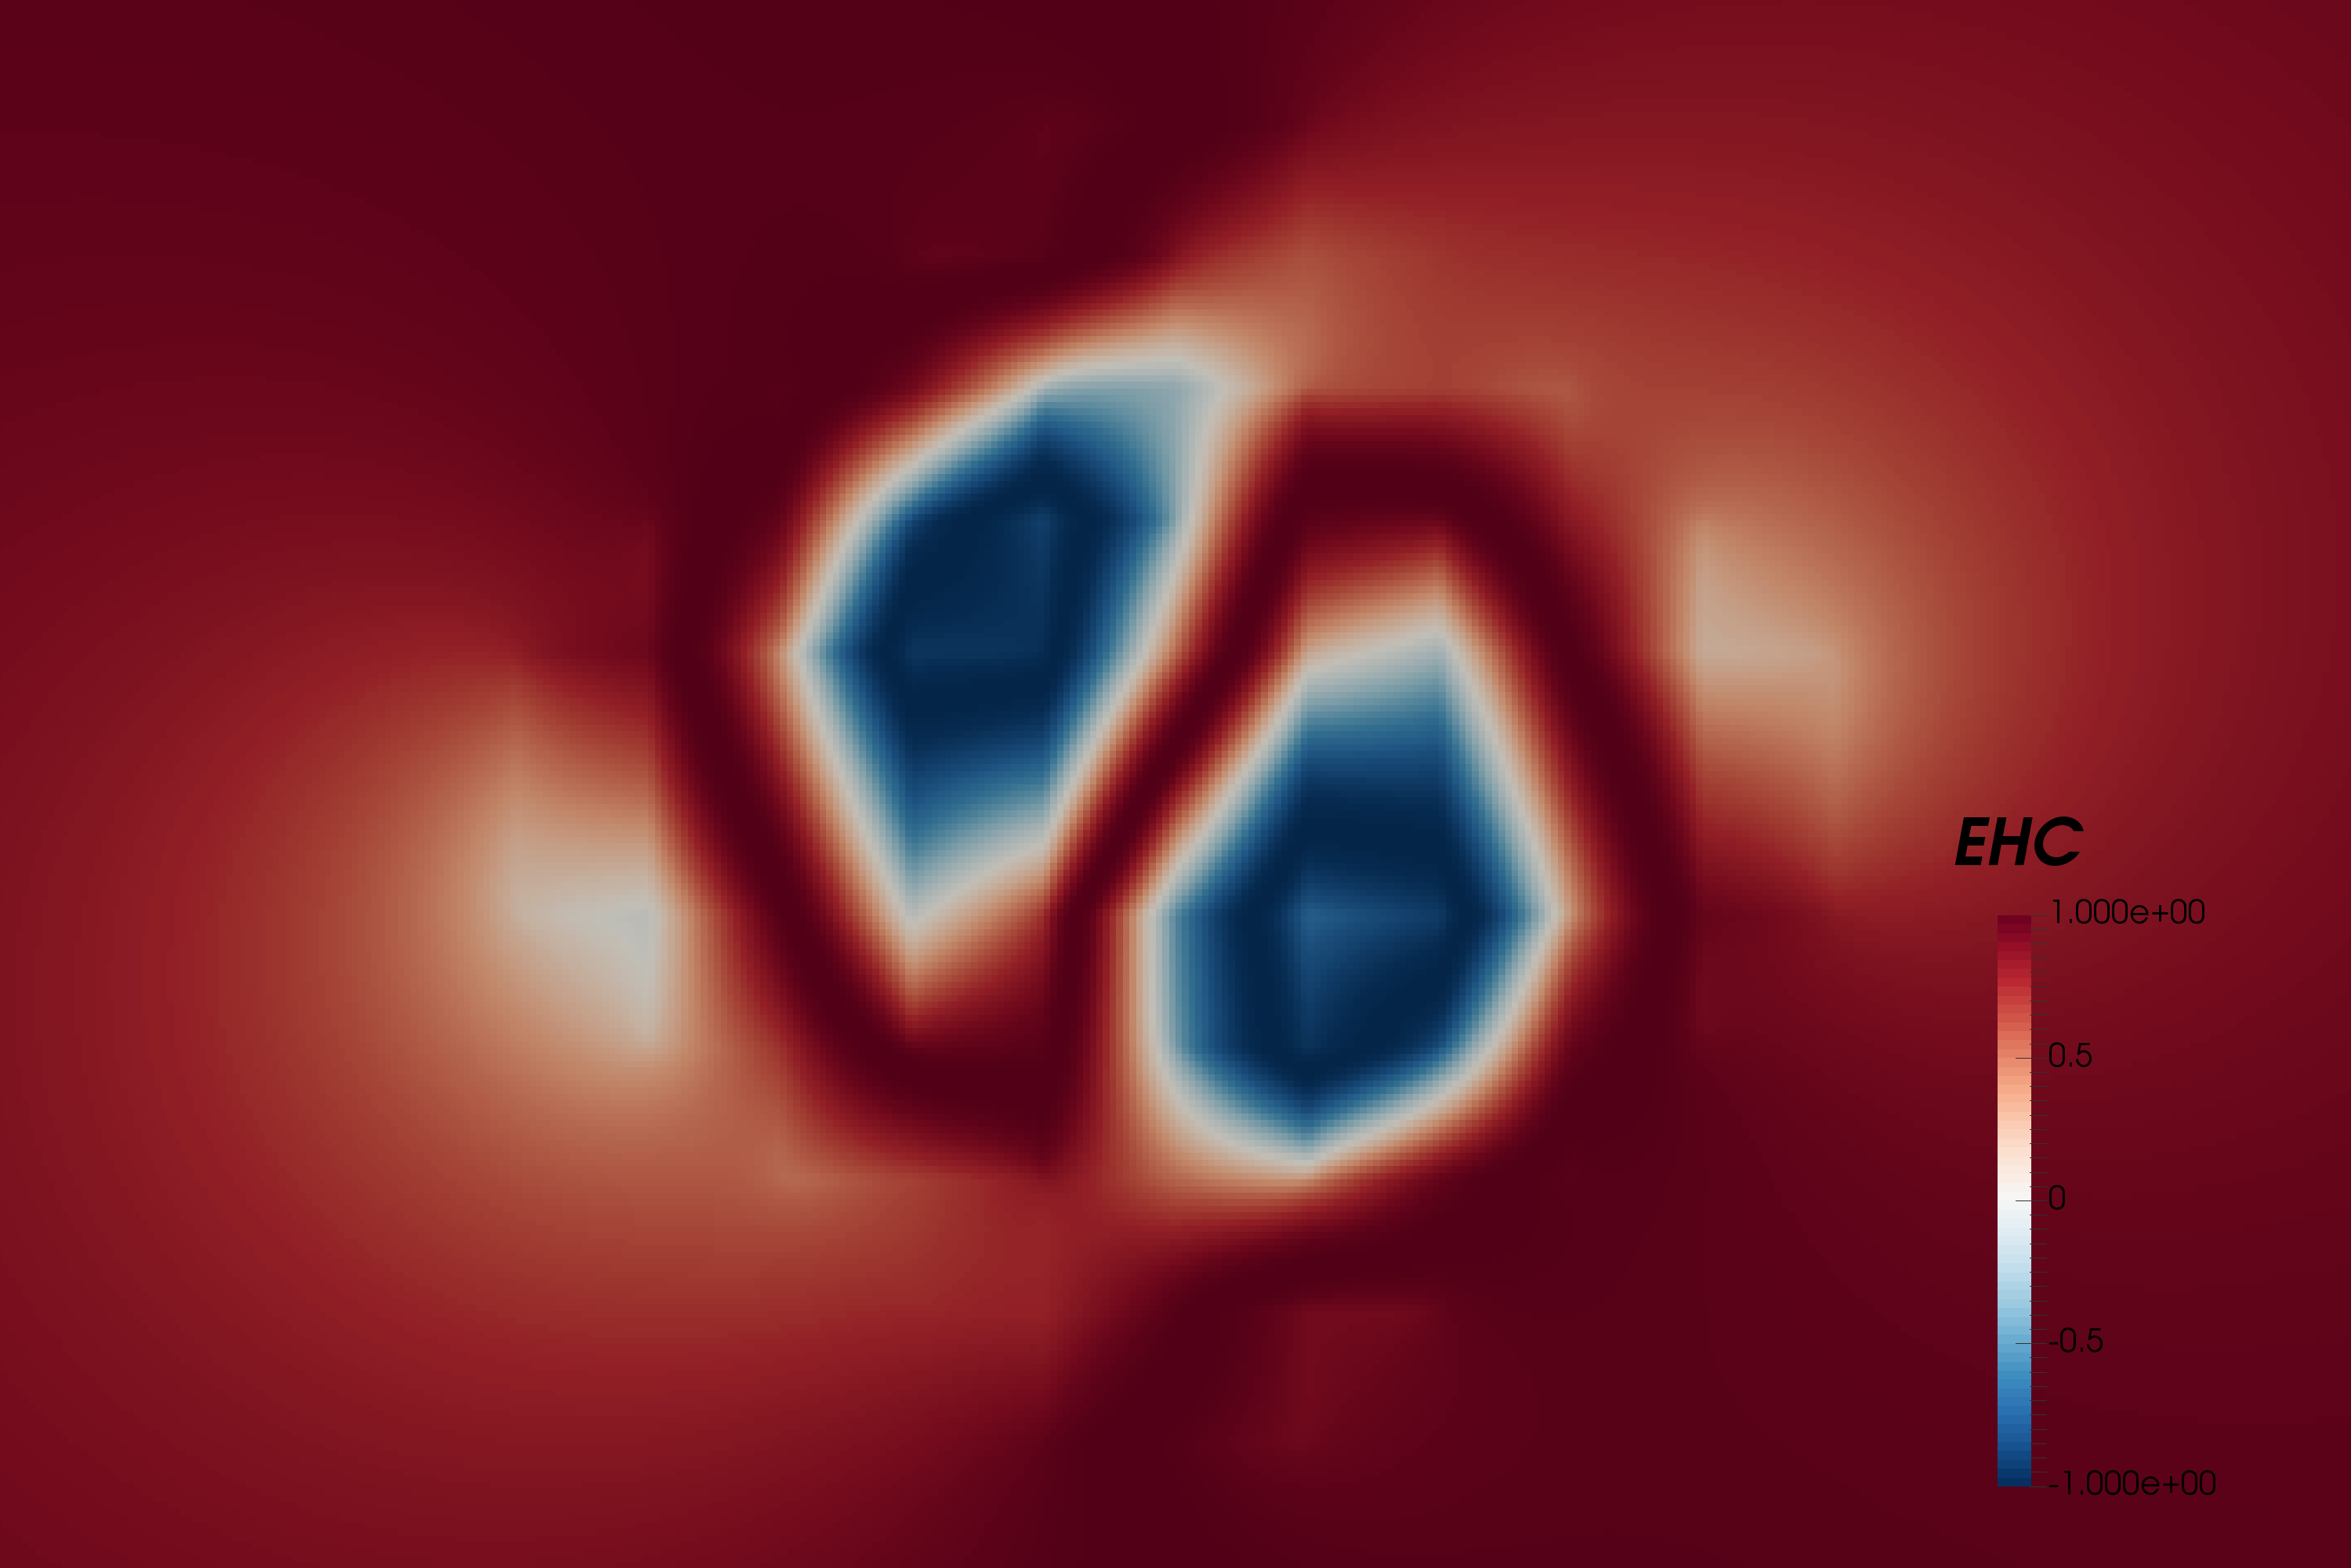
\includegraphics[width=\textwidth]{research-4/figs/fram_i16_f0_-y_EHC.png}
%\caption[Electron holography map of the remanent state when the field is along a hard axis (view from +Y)]{Electron holography map of the remanent state when the field is along a hard axis (view from +Y).}
%\label{FIG_24}
%\end{figure}
%
%\begin{figure}
%\centering
%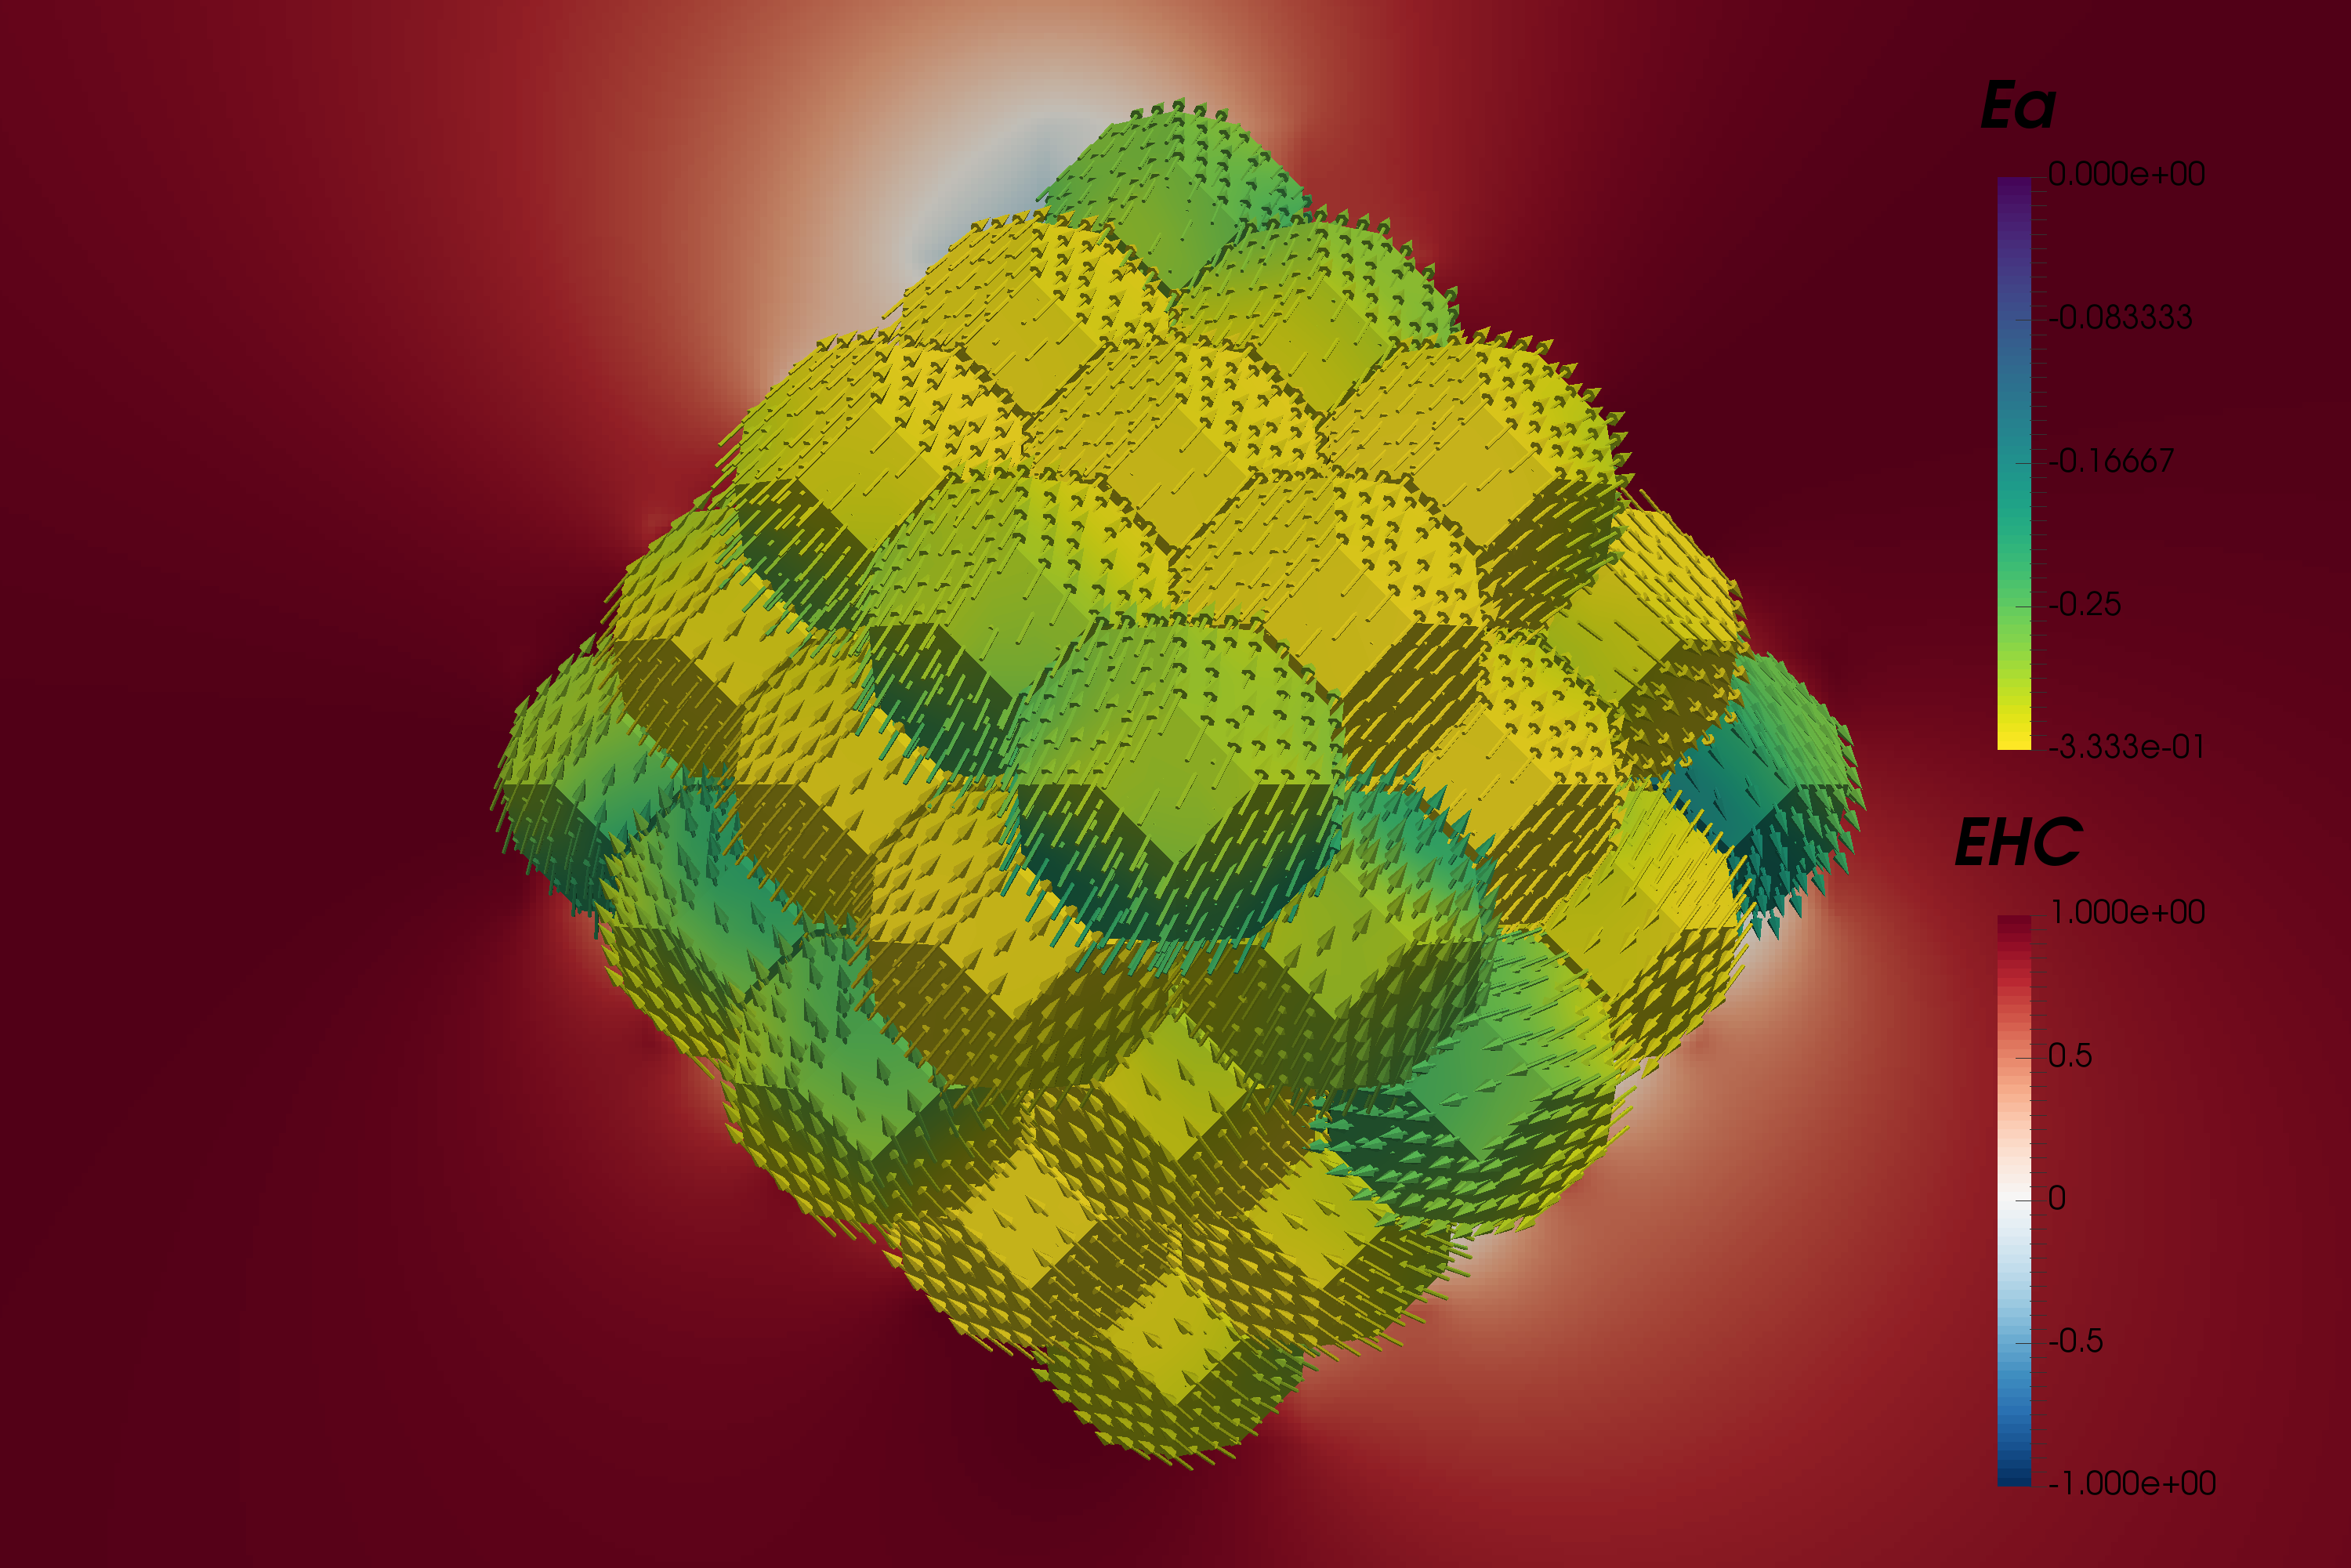
\includegraphics[width=\textwidth]{research-4/figs/fram_i16_f0_-x.png}
%\caption[Remanent state when the field is along a hard axis (view from +X)]{Remanent state when the field is along a hard axis (view from +X).}
%\label{FIG_25}
%\end{figure}
%
%\begin{figure}
%\centering
%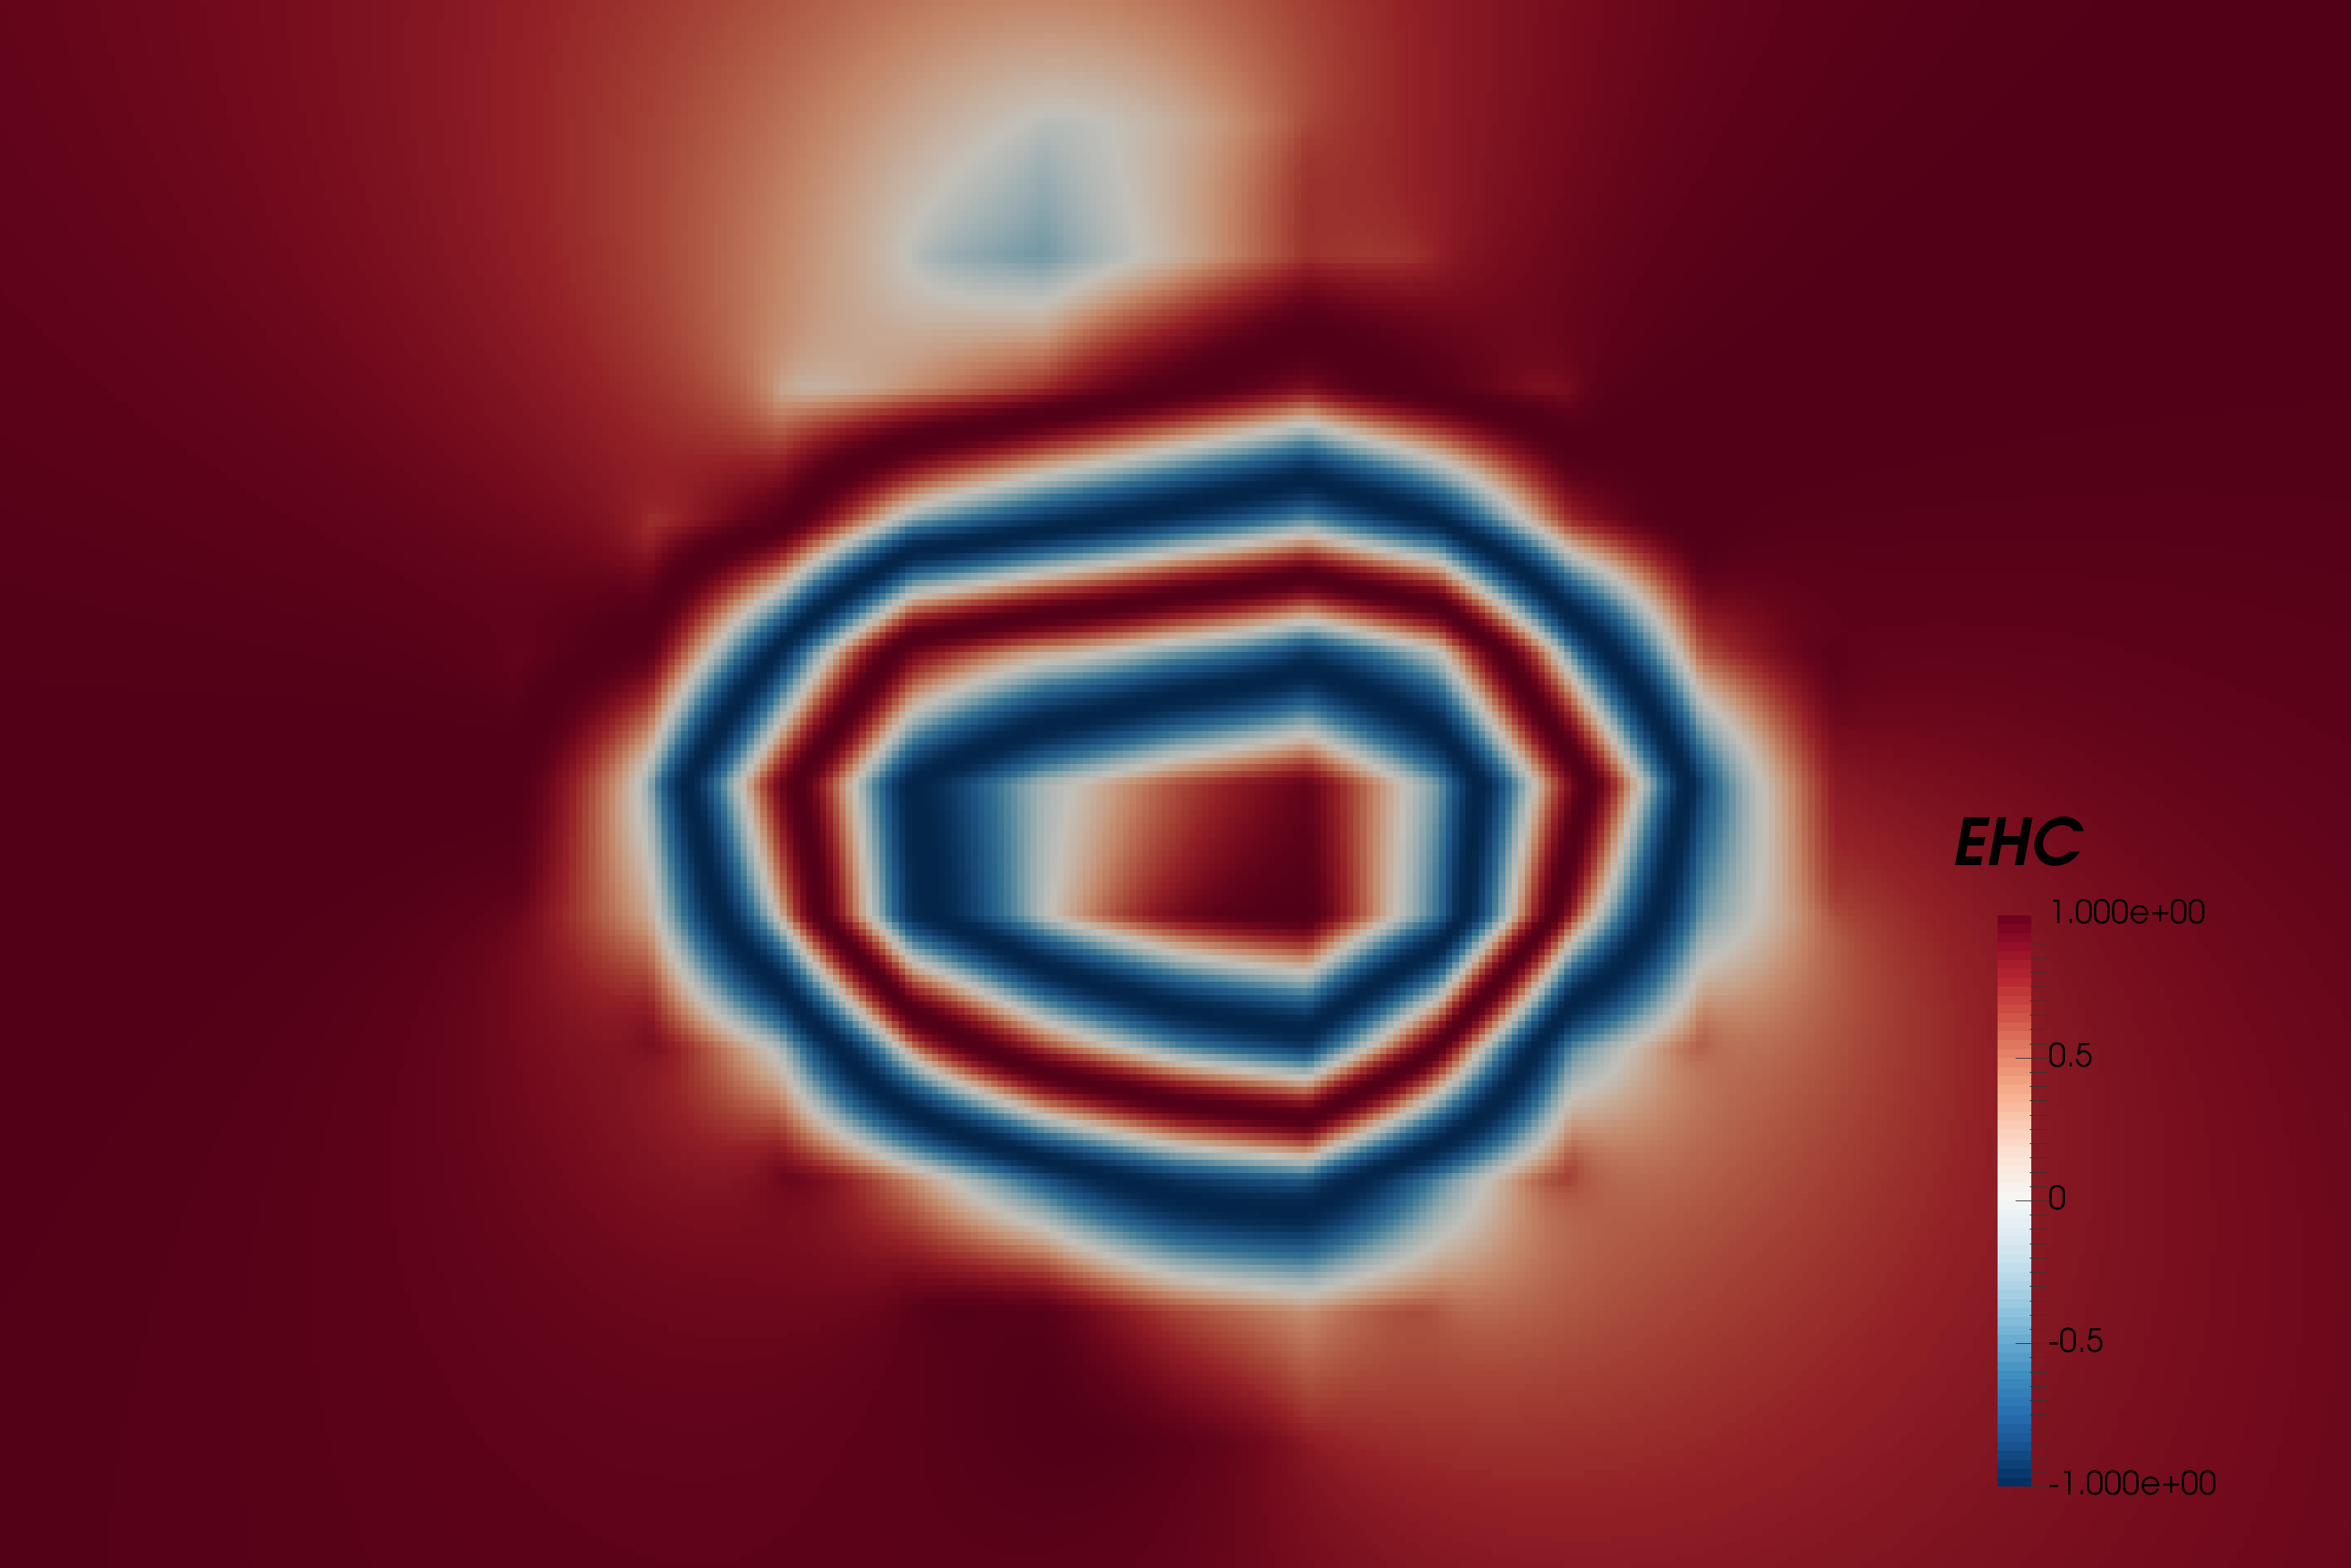
\includegraphics[width=\textwidth]{research-4/figs/fram_i16_f0_-x_EHC.png}
%\caption[Electron holography map of the remanent state when the field is along a hard axis (view from +X)]{Electron holography map of the remanent state when the field is along a hard axis (view from +X).}
%\label{FIG_26}
%\end{figure}
